\chapter{OpenCAPI Characterization}
\label{sec:ch2}

%\todo{
%- Transferring 64B seems wasteful then. Therefore we work here on a cache line granularity.\\
%At tlx 64B data busses are provided. ocapi can transfer 64, 128 or 256B of data by taking multiple cycles over the data bus. power architecture cache line size is 128B. if 64B are requested, the CAPP unit in host cpu fetches the requested cache line of 128B and invalidates one half and transmits the other. transferring less than the cache line size seems wasteful. ask curt if it actually is. maybe in terms of control overhead? Also, do template overhead calculation. can we use all data flits in a single frame if data flits are 128B long?\\
%}

%\todo{MMIO:\\
%\url{https://en.wikipedia.org/wiki/Memory-mapped_I/O} \\
%Used by OpenCAPI. Complementary approach is port-mapped I/O (PMIO) and another option is using dedicated I/O processors. Memory-mapped I/O uses the same address space to address both memory and I/O devices. The memory and registers of the I/O devices are mapped to (associated with) address values. So when an address is accessed by the CPU, it may refer to a portion of physical RAM, but it can also refer to memory of the I/O device. Thus, the CPU instructions used to access the memory can also be used for accessing devices. Each I/O device monitors the CPU's address bus and responds to any CPU access of an address assigned to that device, connecting the data bus to the desired device's hardware register. To accommodate the I/O devices, areas of the addresses used by the CPU must be reserved for I/O and must not be available for normal physical memory. The reservation may be permanent or temporary.\\
%Another good source: \url{http://www.cs.uwm.edu/classes/cs315/Bacon/Lecture/HTML/ch14s03.html} \\
%A lab assignment with Verilog code: \url{http://web.eecs.umich.edu/~prabal/teaching/eecs373-f10/labs/lab3/}\\

%\url{https://en.wikipedia.org/wiki/Address_bus} \\
%"A system with a 32-bit address bus can address $2^{32}$ (4,294,967,296) memory locations."

%Example from the MMIO wiki page:\\
%8-bit processor with 16-bit address lines. 16-bit address line results in 65536 memory locations.
%\begin{equation}
%  $16~bits = 2^{16} = 65536 = 64~kibibytes = 64*1024$
%\end{equation}
%On such a system, the first 32 KiB of address space may be allotted to random access memory (RAM), another 16 KiB to read only memory (ROM) and the remainder to a variety of other devices such as timers, counters, video display chips, sound generating devices, etc. The hardware of the system is arranged so that devices on the address bus will only respond to particular addresses which are intended for them, while all other addresses are ignored. This is the job of the address decoding circuitry, and that establishes the memory map of the system. This memory map contains gaps, which is also quite common in actual system architectures.}
%\todo{INTERRUPT: An interrupt is a signal to the processor emitted by hardware or software indicating an event that needs immediate attention. An interrupt alerts the processor to a high-priority condition requiring the interruption of the current code the processor is executing. The processor responds by suspending its current activities, saving its state, and executing a function called an interrupt handler (or an interrupt service routine, ISR) to deal with the event. This interruption is temporary, and, after the interrupt handler finishes, the processor resumes normal activities. There are two types of interrupts: hardware interrupts and software interrupts. Source: wikipedia}

To get a better understanding of the first OpenCAPI capable system, the system architecture of IBM's POWER9 processor is presented. While OpenCAPI is host architecture agnostic, the standard will be looked at in more detail with respect to the POWER architecture. Several supported accelerator paradigms are shown and finally two initial compatible Xilinx FPGAs are characterized.\\
While our research was being conducted, much of the information on OpenCAPI could only be obtained by talking to the right people, and we hope that this overview may prove useful to others who want to gain a better understanding of this interface.



\section{POWER9 System Overview}

%\todo{- P9 article \url{https://www.nextplatform.com/2017/12/05/power9-to-the-people/}\\
%- interesting about DDR: physically it can either read or write in one cycle. and there is some dead time between read and write because you have to 'turn the DDR around'. memory controller tries to hide this by reorganizing reads and writes. instead of r,w,r,w,etc you want for example r,r,w,w. in contrast, ibm buffer chip does have separate read and write channel. twice as much bw for read compared to write. maybe move this to bandwidth plots at system level.\\
%}

OpenCAPI \cite{opencapi-jeff-preso} is a successor to CAPI 1.0 \cite{capi_ibm} and enables direct attachment of any micro-architecture CPU to coherent user-level accelerators like ASICs and FPGAs and I/O devices such as network and storage controllers. The goal is to have a high-bandwidth and low latency interconnect optimised to enable streamlined implementation of attached devices. The first OpenCAPI enabled system will be in the upcoming POWER9 processor by IBM \cite{thompto-power9}.\\
\autoref{fig:2-p9-system} shows the system architecture of a superset of the various configurations. Depending on the model (SU or SO), there are up to 12 SMT8 or 24 SMT4 cores available accompanied by a collection of various on-chip accelerators such as gzip, 842 compression and AES/SHA cryptography engines. The memory controller supports either eight DDR4 channels or eight "Centaur" memory buffer chips that also act as an off-chip L4 cache. This yields sustained bandwidths of at least \SI{120}{\giga\byte\per\second} and \SI{230}{\giga\byte\per\second}, respectively.\\
POWER9 supports a wide collection of interconnect standards. In total, 48 PCIe Gen 4 lanes are available, which can also be used for CAPI 2.0, for a total half-duplex bandwidth of \SI{96}{\giga\byte\per\second}. Additionally, there are 48 BlueLink lanes operating at \SI{25}{\giga\bit\per\second} servicing either Nvidia NVLink 2.0 attached GPUs or OpenCAPI 3.0 attached devices. This enables an additional \SI{150}{\giga\byte\per\second} of half-duplex bandwidth. Other POWER9 sockets can be attached through an SMP interconnect, by using \SI{16}{\giga\bit\per\second} or \SI{25}{\giga\bit\per\second} lanes. Finally, the cache hierarchy and on-chip interconnect, called the fabric, ties all units together at a maximum bandwidth of \SI{7}{\tera\byte\per\second} \cite{stuecheli-power9}. Due to the coherent nature of the fabric, attached devices can seamlessly communicate with each other and system memory. What sets the POWER9 apart from other vendors is the extended coherency domain across processor cores and attached devices.

%\begin{figure}[H]
%  \centering
%  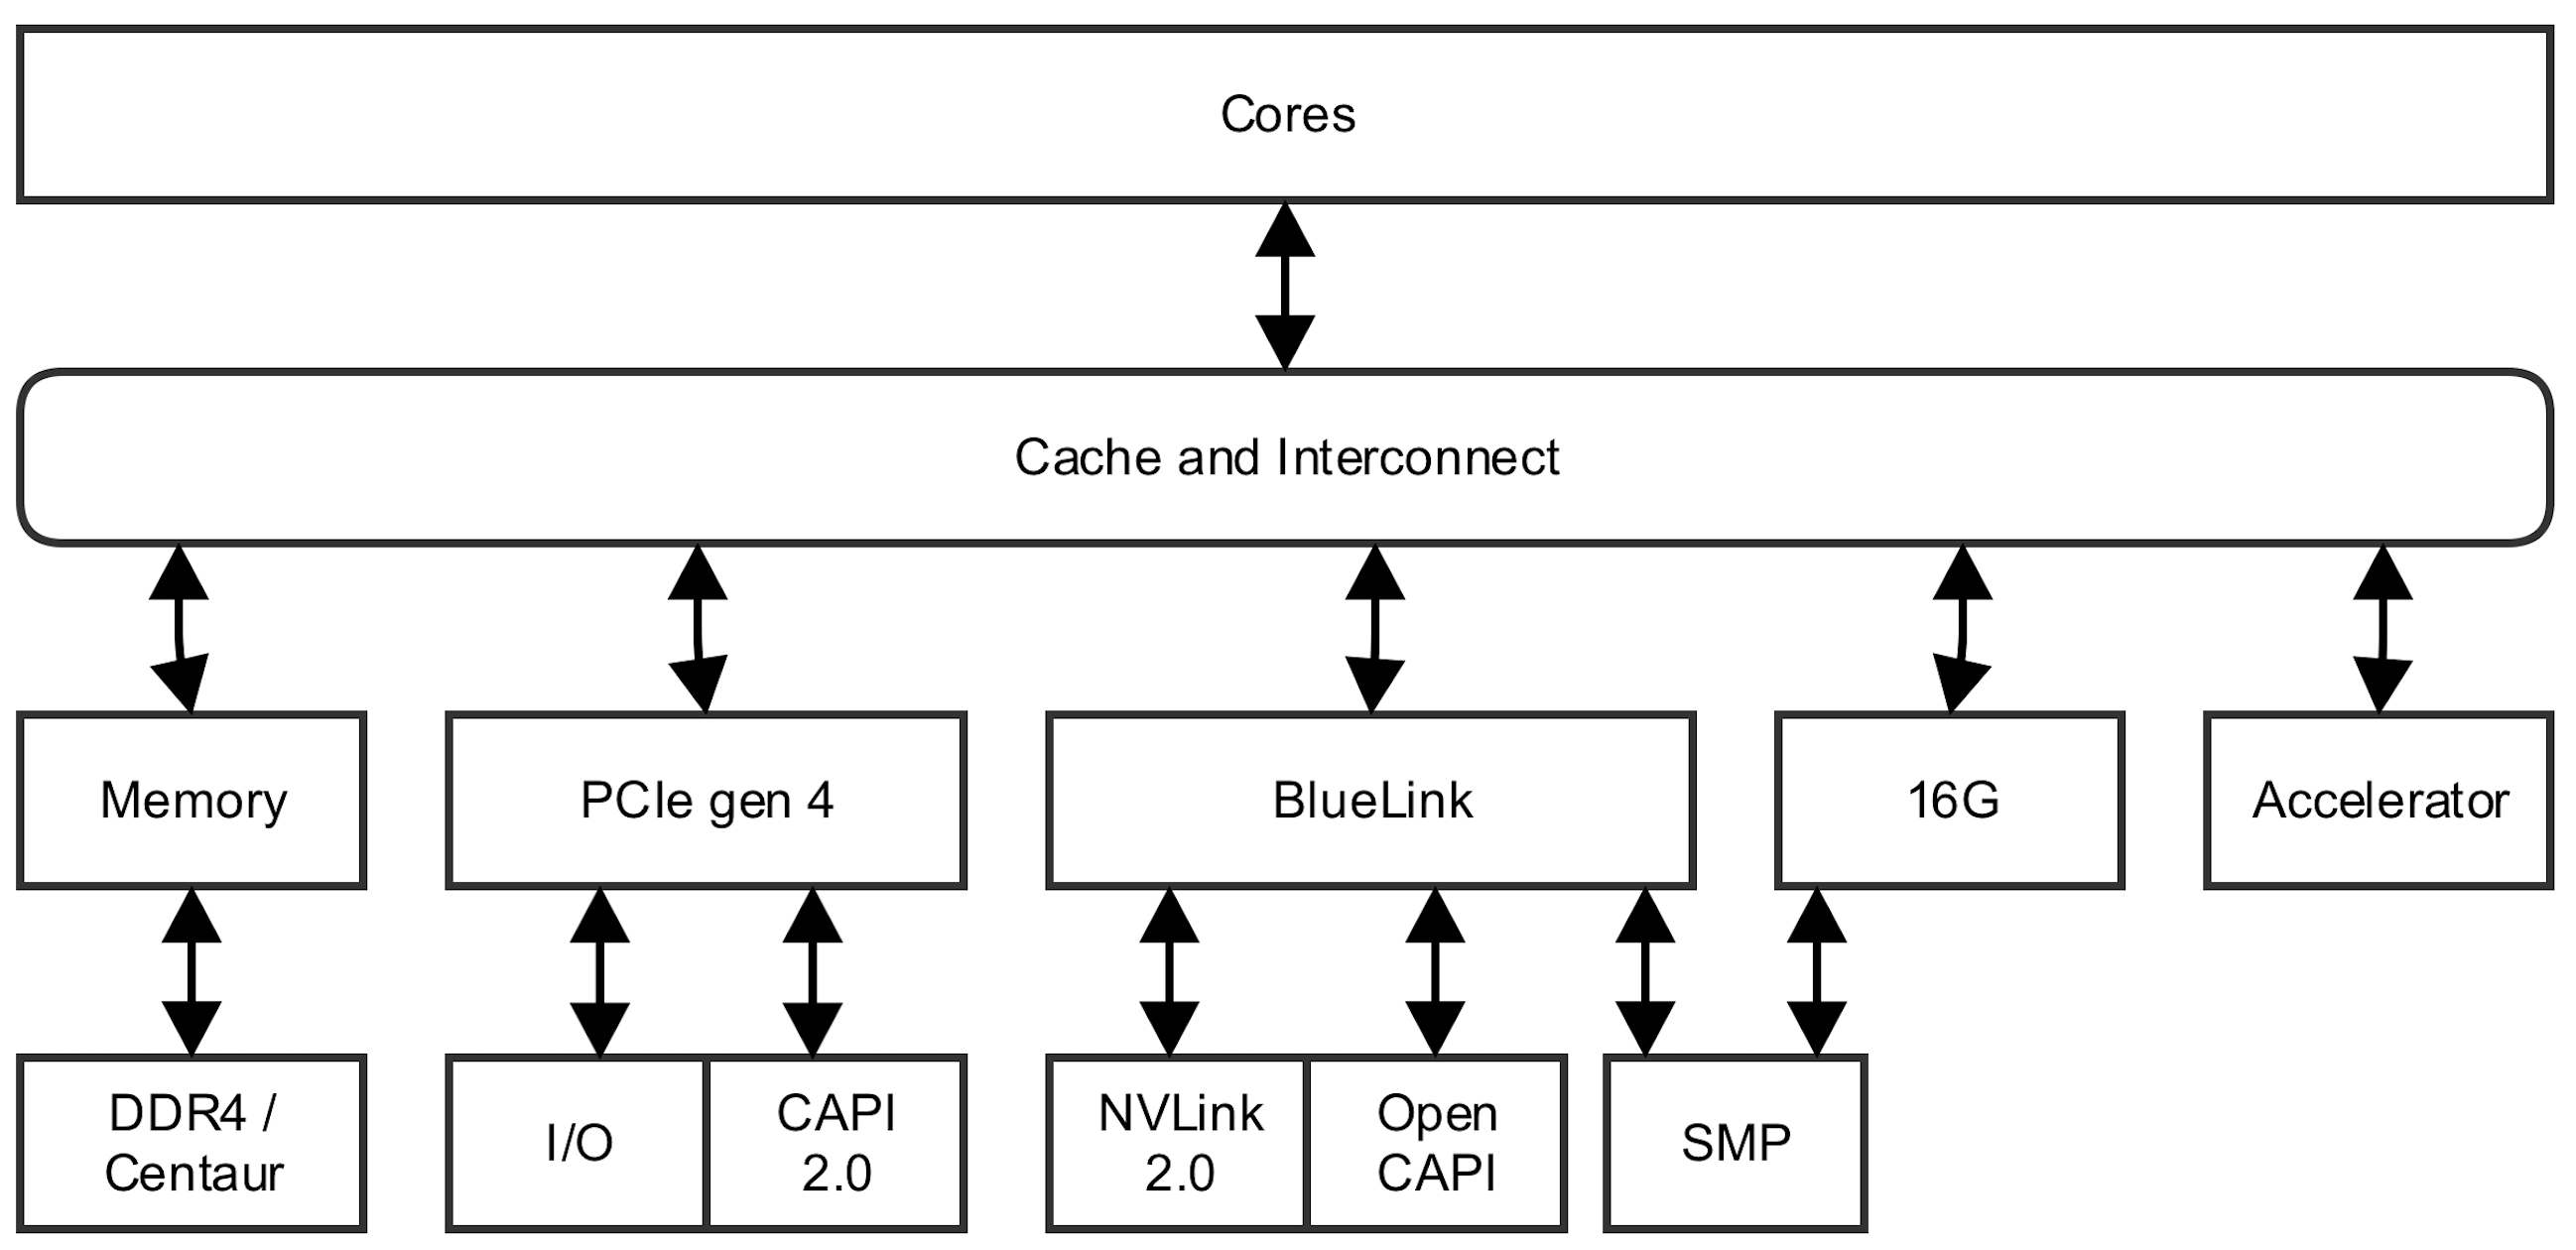
\includegraphics[width=0.80\textwidth]{2-p9-system.png}
%  \caption{System architecture of possible POWER9 configurations \cite{stuecheli-power9}.}
%  \label{fig:2-p9-system}
%\end{figure}
\begin{figure}[h]
  \centering
  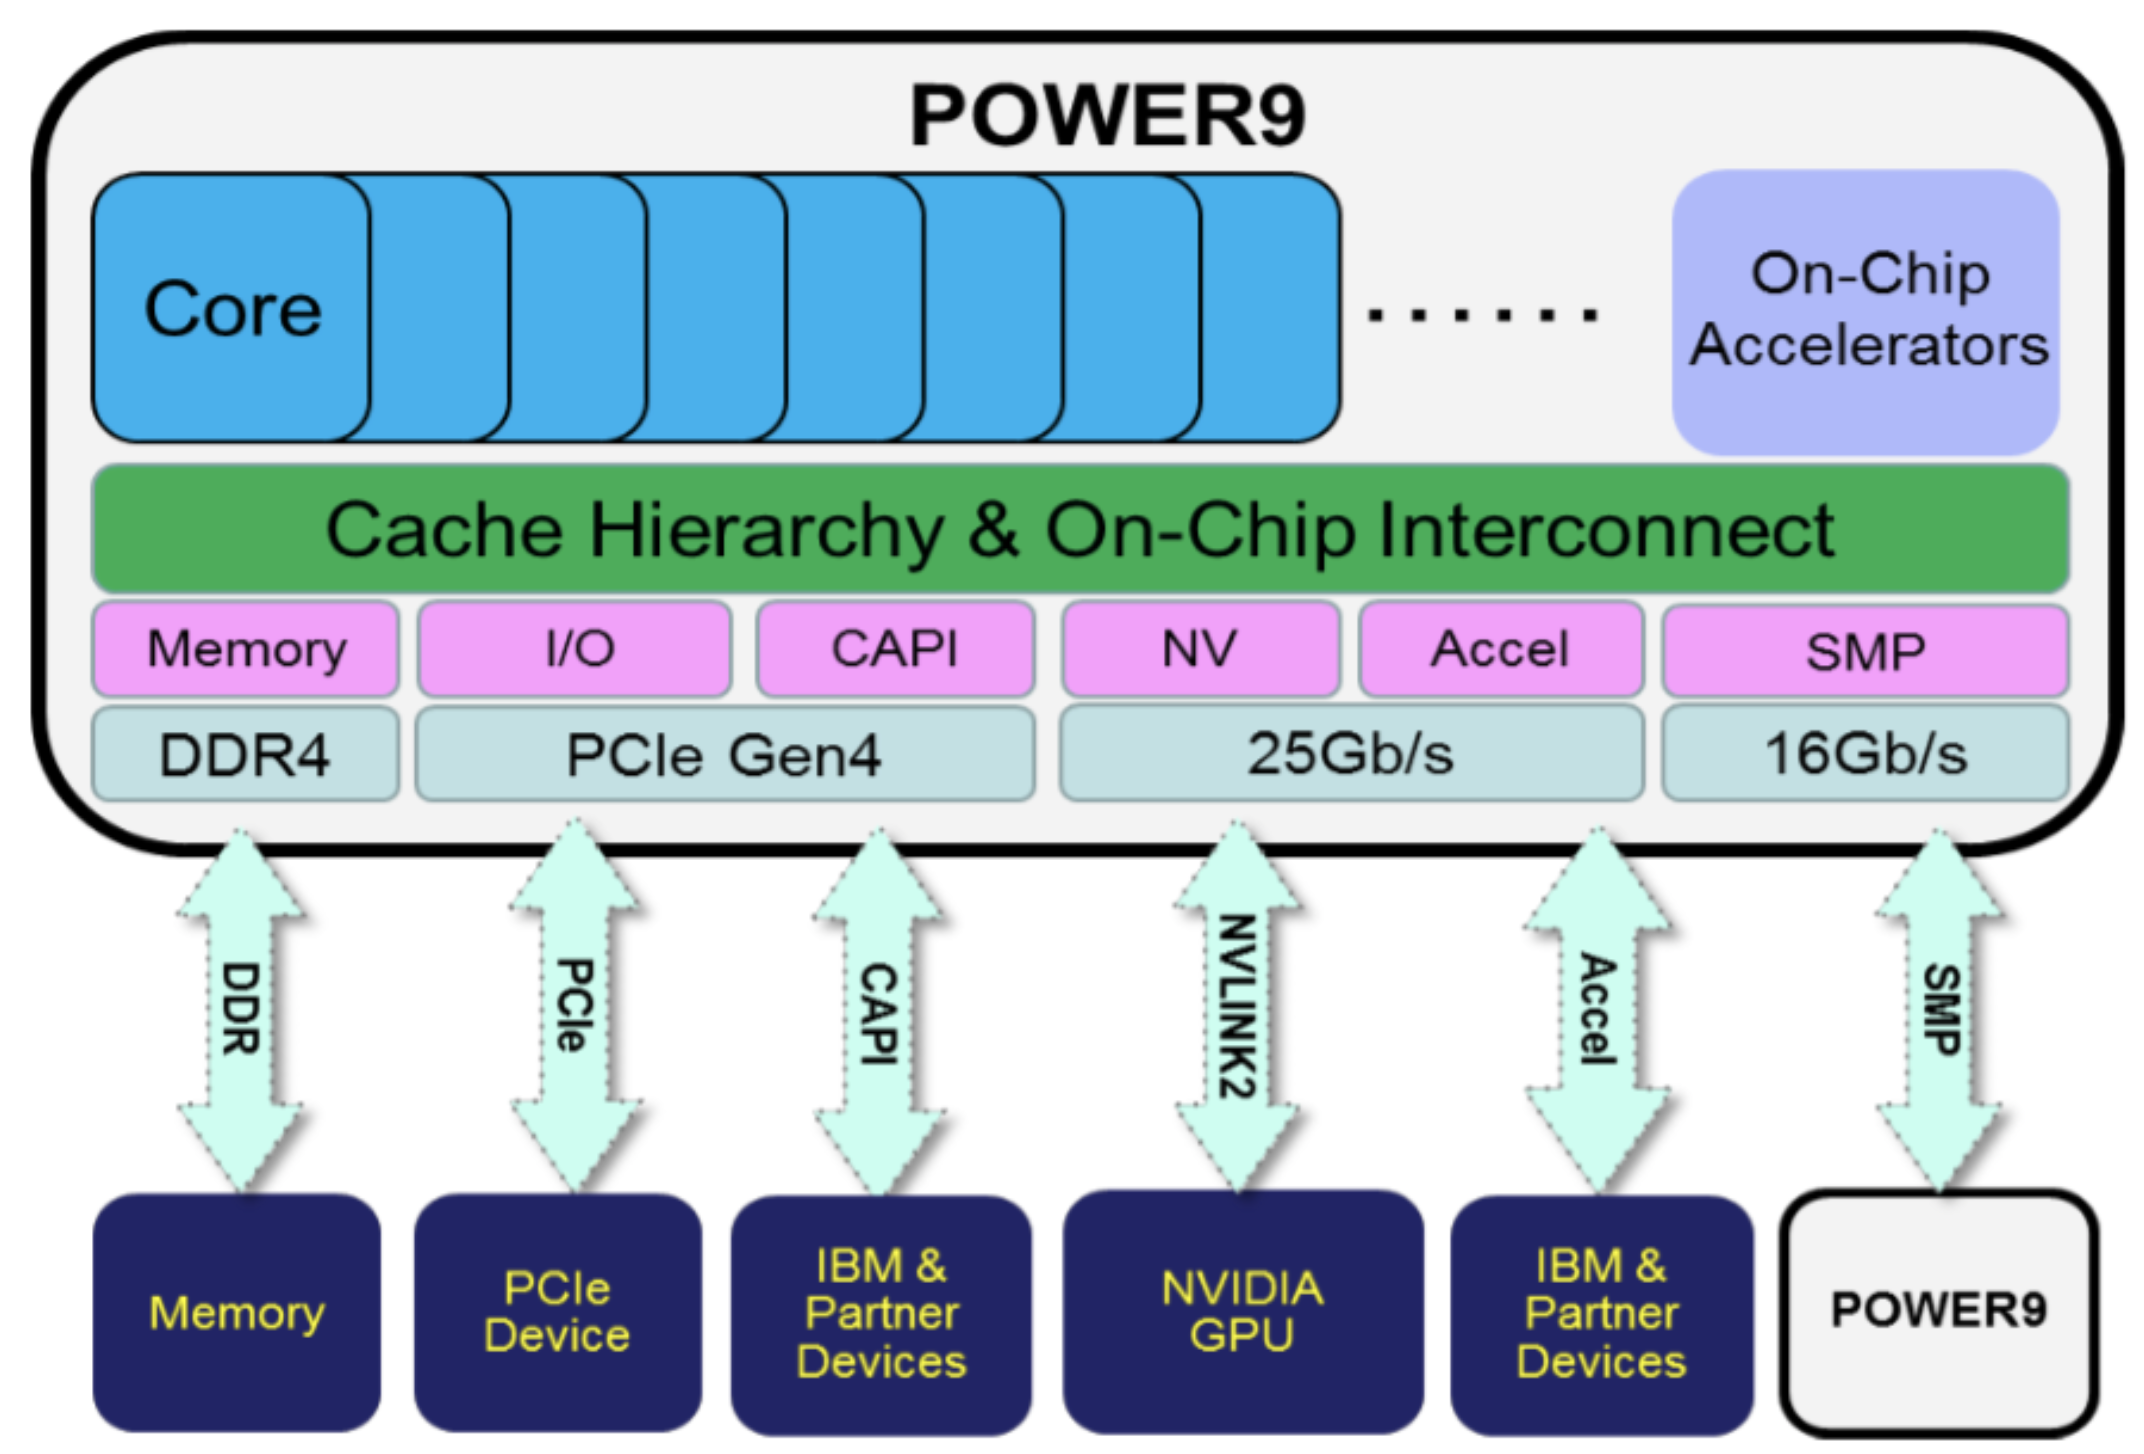
\includegraphics[width=0.70\textwidth]{2-p9-system-2.png}
  \caption{POWER9 system overview \cite{thompto-power9}.}
  \label{fig:2-p9-system}
\end{figure}





\section{OpenCAPI Architecture}
%\todo{- Curt: waiting on official P9 manual for the public.\\
%}

The OpenCAPI architecture consists of several protocol layers divided between the host and attached device \cite{ocapi-dl} \cite{ocapi-tl}. Logic is required on both sides to enable the protocol stack. All logic required for enablement on the host is called the Coherent Accelerator Processor Proxy (CAPP) and is architecture dependent. The CAPP for the POWER architecture is briefly mentioned, but our main focus is on the attached device side. While OpenCAPI also targets emerging storage class memory features, those will not be discussed further and are outside our scope.



\subsection{Protocol Stack}
\autoref{fig:2-ocapi-stack} shows the OpenCAPI stack that is partly located on the host CPU and partly on the attached device. OpenCAPI is a credit-based point-to-point protocol. The link has a number of credits that are consumed when data is transferred in order to throttle traffic. While in essence there are no differences from the point of view of the stack between attaching an ASIC or FPGA, only FPGAs will be considered due to the aim of the thesis.\\
In comparison to CAPI 1.0, the PSL is now located in the host processor, which removes the logic overhead within the FPGA. Complexities of coherence and virtual addressing are implemented on the host CPU to simplify the design of attached devices and facilitate interoperability across different CPU architectures. Due to the coherent nature, attached devices can operate natively within an application's user space. This allows attached devices to fully participate in an application without involvement or overhead of the kernel \cite{stuecheli-power9}.\\
The stack consists of several layers that are briefly introduced. Messages (packets) can be initiated by either the CAPP (host) or AP (AFU) and are called CAPP or AP command packets, respectively (see Section \ref{sec:packets}). When the Transaction Layer on either side receives a command packet, a response packet has to be sent back, called a CAPP or AP response packet, respectively. Note that while the stack looks symmetric, the transaction layers on both sides are very different, since their implementation depends on the host architecture and AFU protocol, respectively.

\begin{itemize}
  \item{\textbf{Host Protocol Layer} is the coherent connection to the rest of the host. The implementation is host architecture dependent and all required logic to implement OpenCAPI is called the CAPP (see Section \ref{sec:capp}).}
  \item{\textbf{Transaction Layer (TL)} converts host protocol-specific requests into CAPP command packets and generates and handles CAPP response packets. Internally it consists of a framer and parser.
  \begin{itemize}
    \item{\textbf{Framer} packetizes CAPP commands and responses along with credit packets into control flits according to various packing templates. Different templates exist since packets have different sizes. Control and data flits are sent to the DL while ensuring frame order.}
    % Flow control.
    % Error handling.
    % Manages virtual channels, virtual queues, and service queues associated with the virtual channels. Order is retained within virtual channels. See service queue and virtual queue in this glossary.
    \item{\textbf{Parser} receives DL frames consisting of control and data flits (see Section \ref{sec:frame}). It parses the control flit into AP command and response packets and returns credits to the Framer. The AP packets are passed to the host.}
  \end{itemize}
  }
  \item{\textbf{Data Link Layer (DL)} converts DL frames, consisting of a single control flit and between zero and eight data flits, to PHY transmittable data.}
  \item{\textbf{Physical Layer (PHY)} represents the actual connector and link on the host CPU. Each lane operates at \SI{25.78125}{\giga\hertz}. For the POWER9, each PHY brick consists of eight duplex lanes.}
\end{itemize}

In opposite order, the PHYX, DLX and TLX layers present on the FPGA act similarly to their host counterparts, where X stands for eXternal. However, the TLX does not handle responses. This has to be taken care of by the APL or AFU, depending on implementation.\\
An additional layer present on the FPGA is the AFU Protocol Layer (APL). This is an optional layer and an AFU can also directly interface with the TLX if desired. An example of this layer could be a bridge to AXI, the \textit{de facto} standard for FPGAs, similarly to the AXI4 to CAPI 1.0 adapter by Xilinx \cite{xilinx-xapp1293}. On the other side the APL interfaces with the Attached Functional Unit (AFU), or accelerator.

\begin{figure}[h]
  \centering
  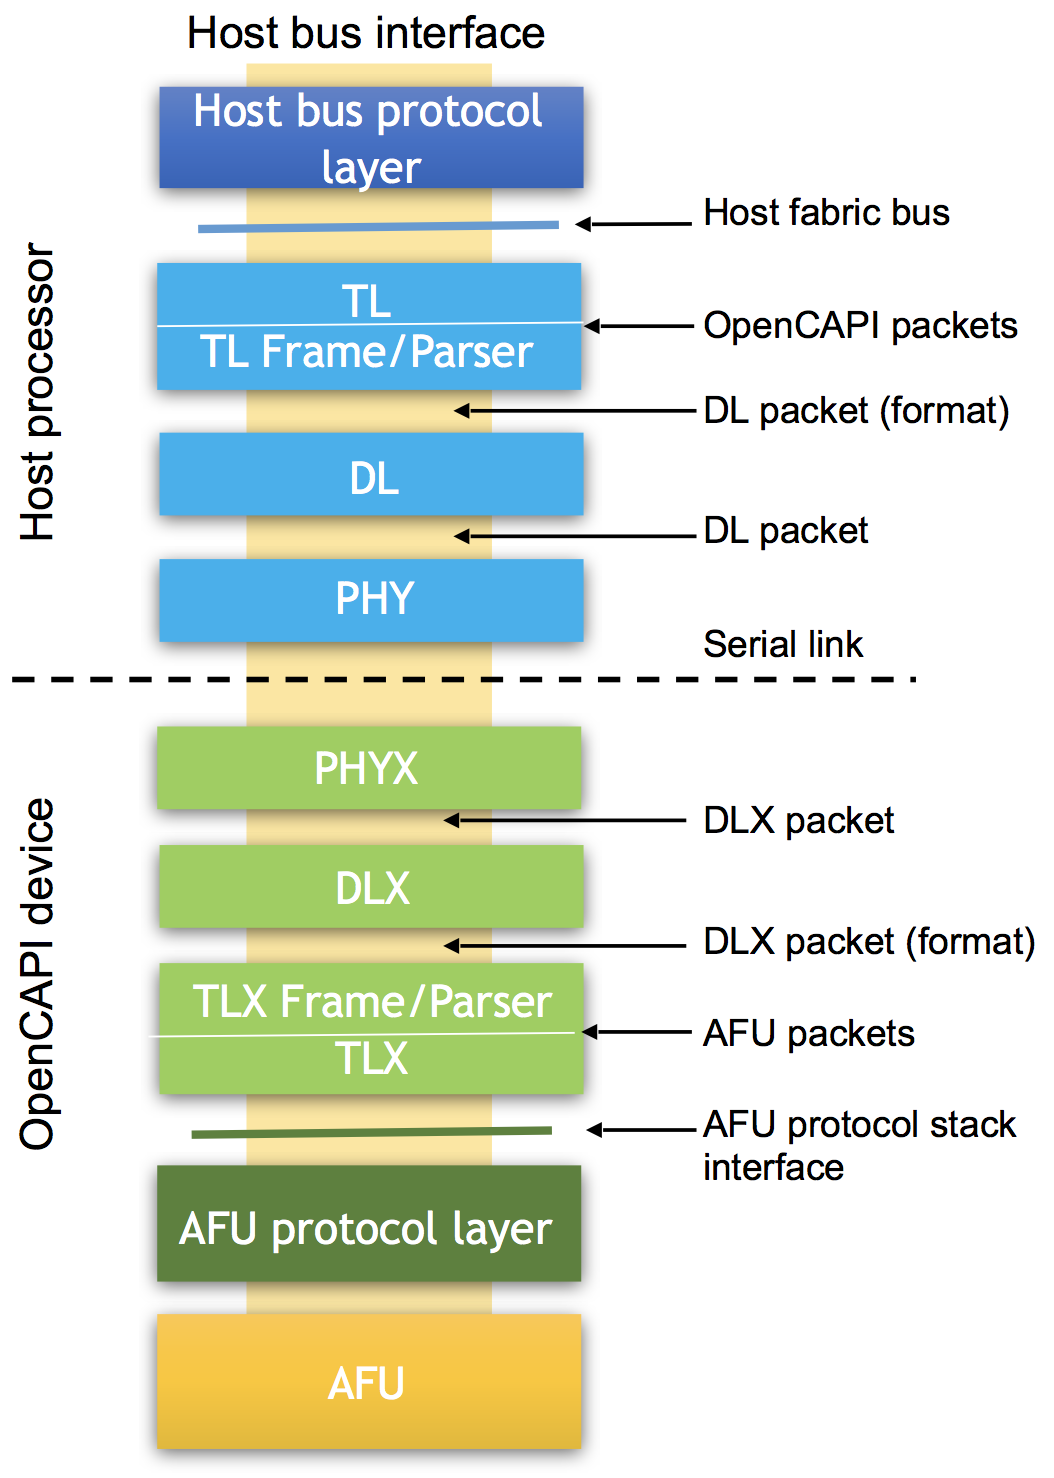
\includegraphics[width=0.55\textwidth]{2-ocapi-stack.png}
  \caption{The OpenCAPI stack from host to attached device \cite{opencapi-enablement}.}
  \label{fig:2-ocapi-stack}
\end{figure}



\subsection{Data Link Layer Frame Format}
\label{sec:frame}
Typically, packets are broken up in smaller pieces called flits, which stands for FLow control unIT. The first flit is the packet header and contains control information. Other flits, corresponding to the same packet, are data flits. In the context of OpenCAPI, the network packet is called a (DL) frame and the term packets is reserved for CAPP and AP commands and responses. The term TL packets acts as an umbrella for all different packets.\\
Both the TL and TLX framer and parser work with DL frames \cite{ocapi-dl}. A DL frame consists of one control flit and between zero and eight data flits, where at most four data flits belong to a single TL packet. Every flit is 64 bytes in size. Flits are transmitted starting at the lowest order control flit bytes and continuing in increasing address order. After that, the data flits are transmitted similarly. A control flit consists of an 8 byte DL content field and 56 bytes of TL packets, packed according to a predefined packing template. The OpenCAPI 3.1 TL specification \cite{ocapi-tl} adds a datum field to the control flit which embeds data smaller than 64 bytes within the control flit for improved frame utilization.

The DL content field contains both DL and TL generated subfields. Important are the DL injected CRC and TL injected TL template subfields. The CRC covers both the current control flit and the data flits from the previous control flit. Upon detection of an error, all data flits from the previous control flit are invalid and the transmitter is requested to replay the data flits. The final control flit never has any data flits, since it has to validate the last data flits using its CRC.\\
\autoref{fig:2-ocapi-frame} shows several DL frames and their respective control and data flits. The same colored flits indicate how a CRC in the DL content field corresponds to the data flit(s) from the previous control flit. The TL template subfield specifies the location of TL packets in the remainder of the control flit. The 56 bytes, or 448 bits, of TL packets in the control flit consist of sixteen, 28 bits, slots. TL packets differ in length and can consume between one and six slots per packet. Different package templates exist that indicate how many TL packets are present and how many slots they consume.

%DL: data run length, ACK count, CRC
%TL: bad data flit indication, TL template

\begin{figure}[h]
  \centering
  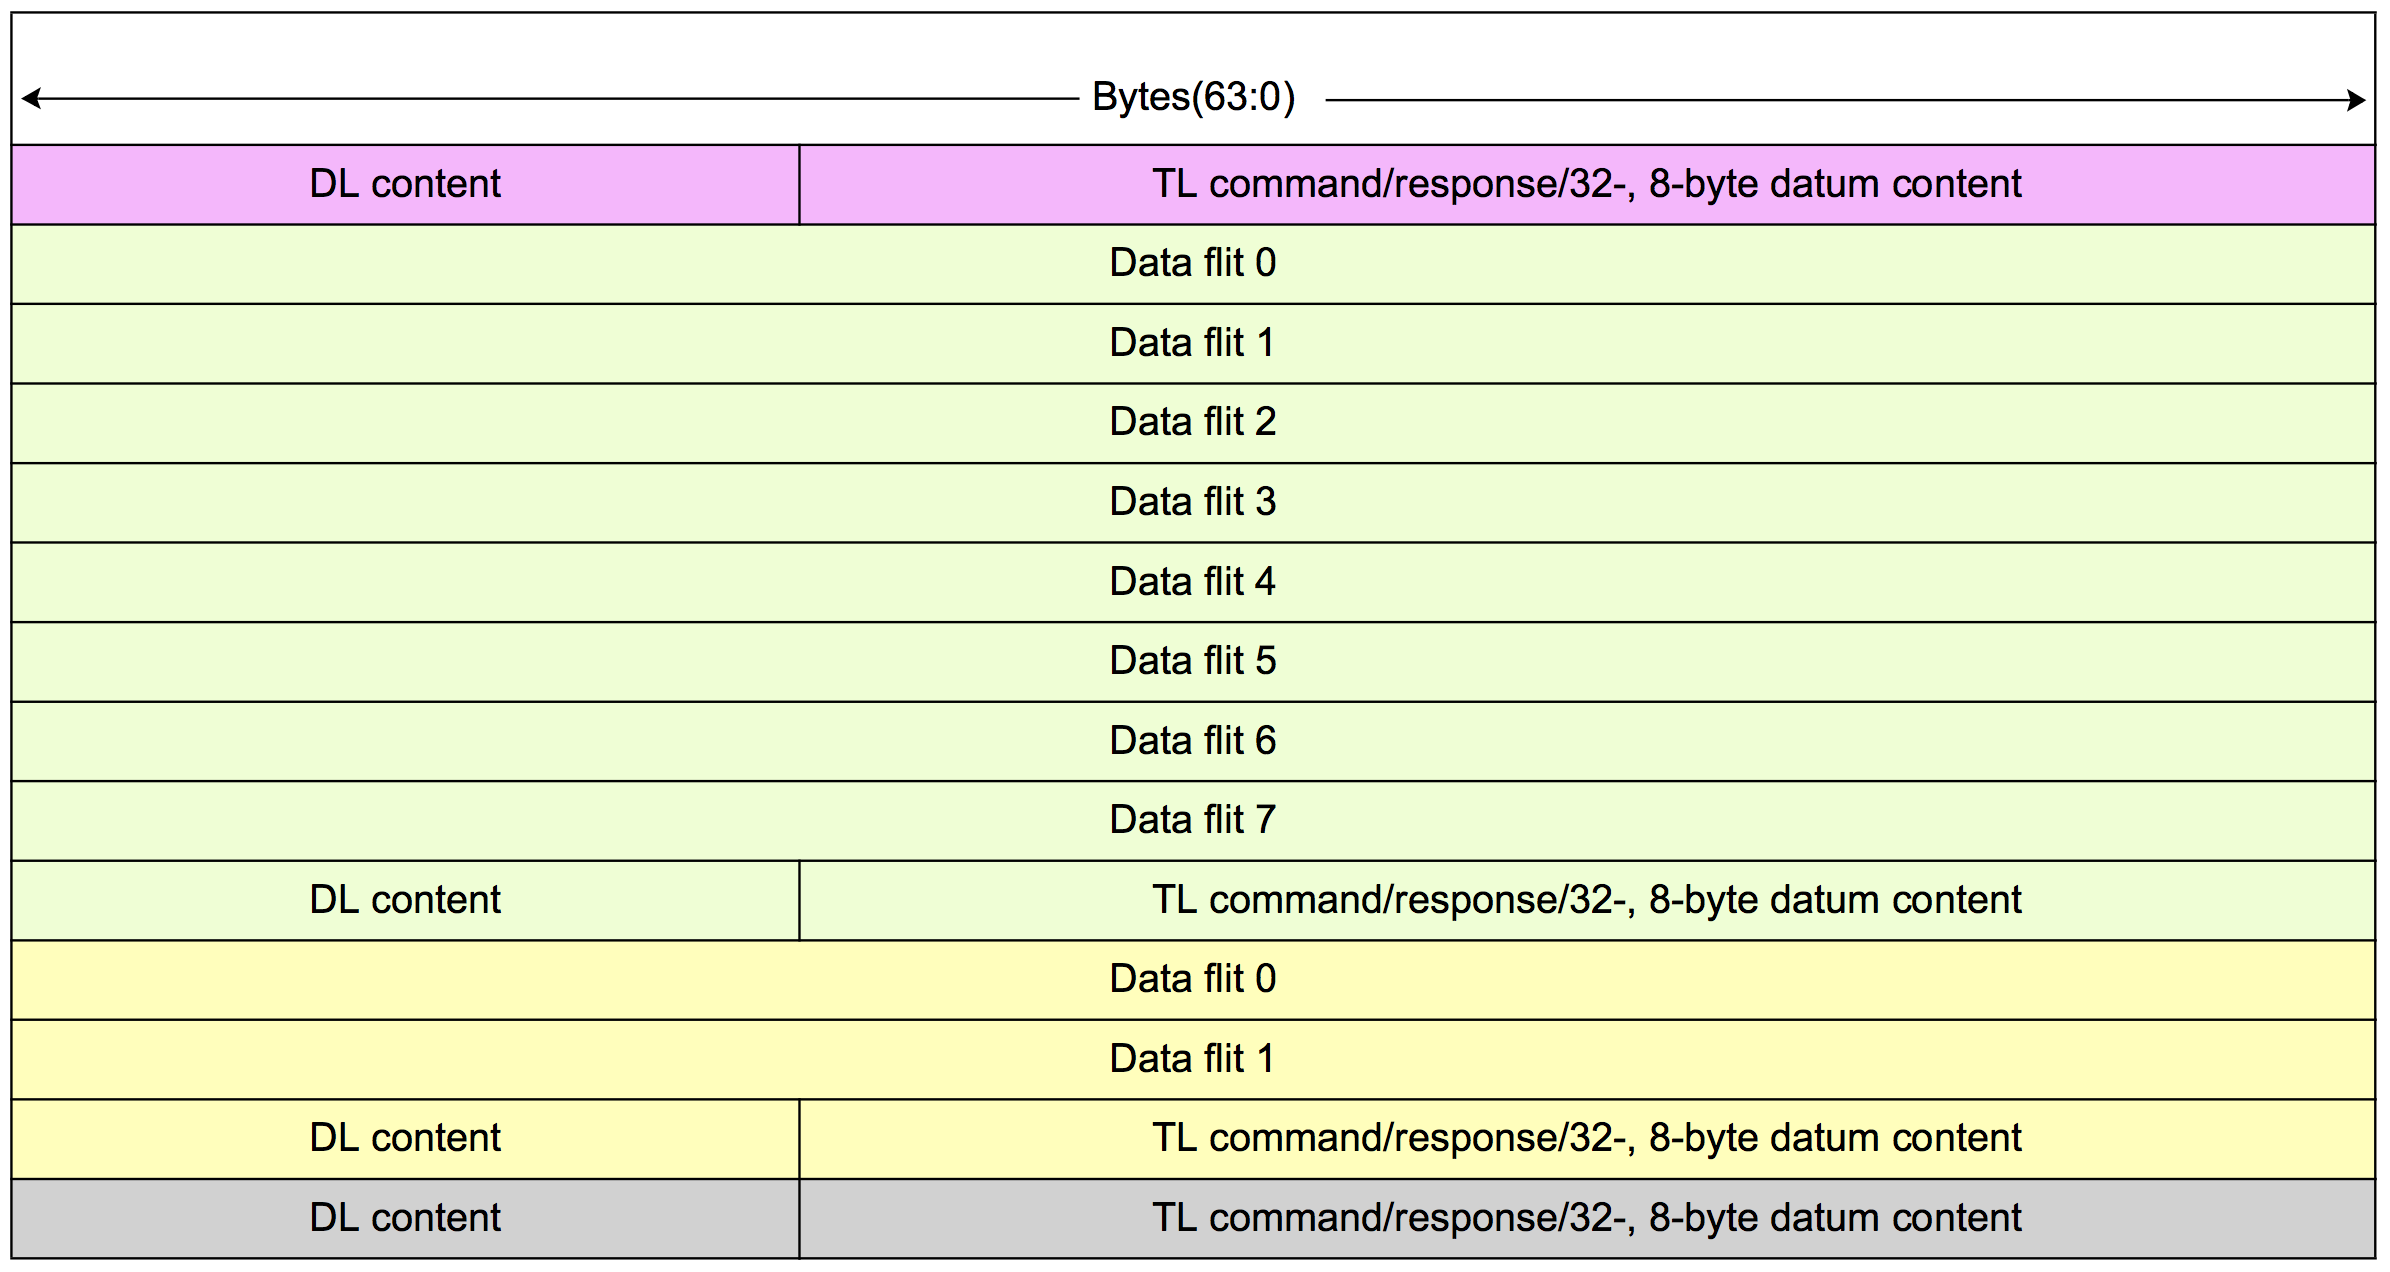
\includegraphics[width=0.85\textwidth]{2-ocapi-frame.png}
  \caption{Example of several DL frames showing the CRC control and data flit coverage \cite{ocapi-tl}.}
  \label{fig:2-ocapi-frame}
\end{figure}



\subsection{Transaction Layer Packets}
\label{sec:packets}
TL packets are control instructions that can be sent within a control flit \cite{ocapi-tl}. Depending on which side of the OpenCAPI link initiated the packet, the prefix CAPP (for the host) or AP (for the AFU) is used. There are several different types of packets, depending on the source. The host can issue from the following categories of commands. Bear in mind that each command requires a response (not listed below).
\begin{itemize}
  \item{\textbf{Address Translation} The host notifies the AFU that a previous address translation request has been completed.}
  \item{\textbf{Configuration Space} Reading and writing to the configuration space of the AFU is supported with specific commands.}
  \item{\textbf{Interrupt} The host updates the AFU regarding a previous interrupt request.}
  \item{\textbf{Memory Access} The host can read and write AFU memory at 64, 128 or 256 bytes data sizes at a time. It supports partial reads and partial and byte-enabled writes.}
  \item{\textbf{Metadata} An optional and implementation specific field to hold metadata for a data block held in memory.}
\end{itemize}
The AFU supports a different set of command categories.
\begin{itemize}
  \item{\textbf{Address Translation} The AFU can request address translation prefetching for an EA to warm up the address translation cache. This allows an accelerator to reduce translation latency when using a new page.}
  \item{\textbf{Assign acTag} The Address Context Tag (acTag) is used to index a host table containing the associated BDF and PASID. The BDF and PASID are used for address translation authorization and operation validation.}
  \item{\textbf{Atomic Operations} are supported to host memory (read, write, read-write). An accelerator can perform atomic operations in the same coherent domain just like any other host processor thread. Multiple variations are supported by hardware.}
  \item{\textbf{Interrupt} The AFU can request interrupt service on the host.}
  \item{\textbf{Memory Access} Currently, the AFU has no coherent cache. Therefore, read commands have a suffix to indicate no intent to cache. A coherent cache will be supported in OpenCAPI 4.0. A partial read is supported, as well as byte-enabled and partial writing.}
  \item{\textbf{Wake Host Thread} is an efficient low-latency mechanism used for communication between the host and attached device instead of either interrupts or host polling mechanism of host memory.}
\end{itemize}

Both the CAPP and AP side support a response packet for returning credits. As mentioned earlier, these are used for flow control.



\subsection{Coherent Accelerator Processor Proxy}
\label{sec:capp}

%\todo{- what are pages?\\
%}

The CAPP, in a host architecture agnostic context, contains all logic required on the host to enable OpenCAPI. \autoref{fig:2-ocapi-host-1} shows a possible system architecture where the CAPP is coherently connected to the rest of the host. An OpenCAPI device is then connected to the other side of the CAPP. Note that module names used here might change in the official documentation.\\
\autoref{fig:2-ocapi-host-2} shows CAPP implementations for the POWER9 \cite{curt}. It includes the OpenCAPI Processing Unit (OPU) and Nest Memory Management Unit (nMMU). The OPU consists of three stacks and each stack services two physical bricks of eight lanes. This brings the total to 48 lanes. Each stack consists of an XSL, and the DL and TL layers. The XSL handles address translation and has a dedicated ERAT/TLB of 64 entries and each entry represents a \SI{64}{\kilo\byte} page. Two stacks support OpenCAPI and are statically configured to use either OpenCAPI or NVLink 2.0 DL and TL layers, that in turn are connected to the PHY. The nMMU handles translation requests from other units than the CPU cores. It has its own ERAT/TLB with 8192 page entries, significantly more than the XSL.

%\begin{figure}[H]
%  \begin{subfigure}{0.5\textwidth}
%    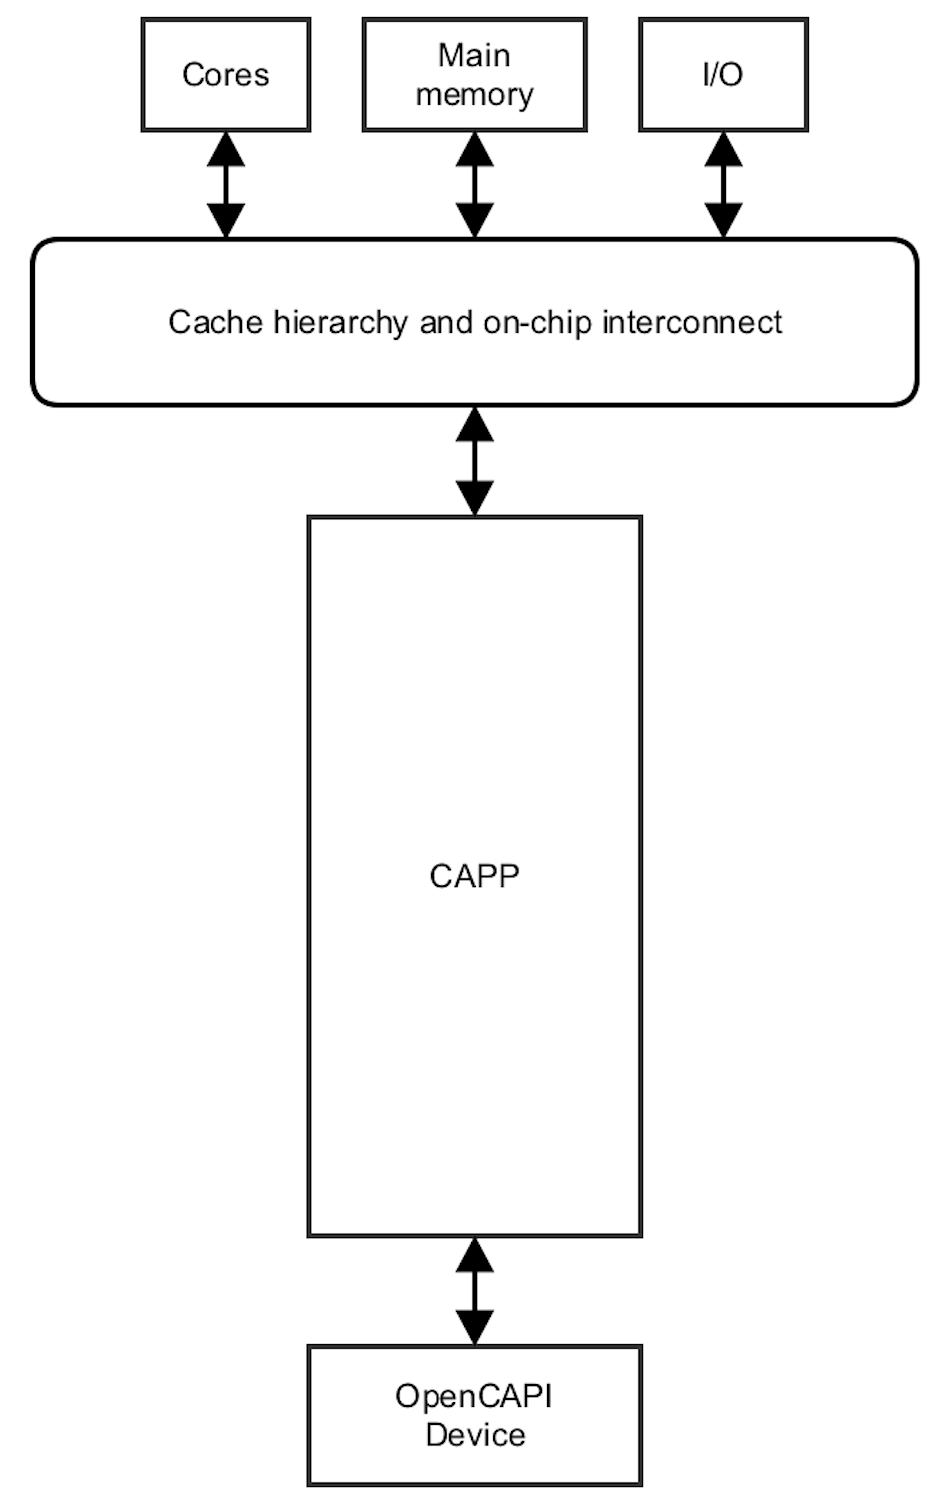
\includegraphics[width=0.6\linewidth]{2-ocapi-host-1.png}
%    \caption{Host architecture agnostic.}
%    \label{fig:2-ocapi-host-1}
%  \end{subfigure}
%  \begin{subfigure}{0.5\textwidth}
%    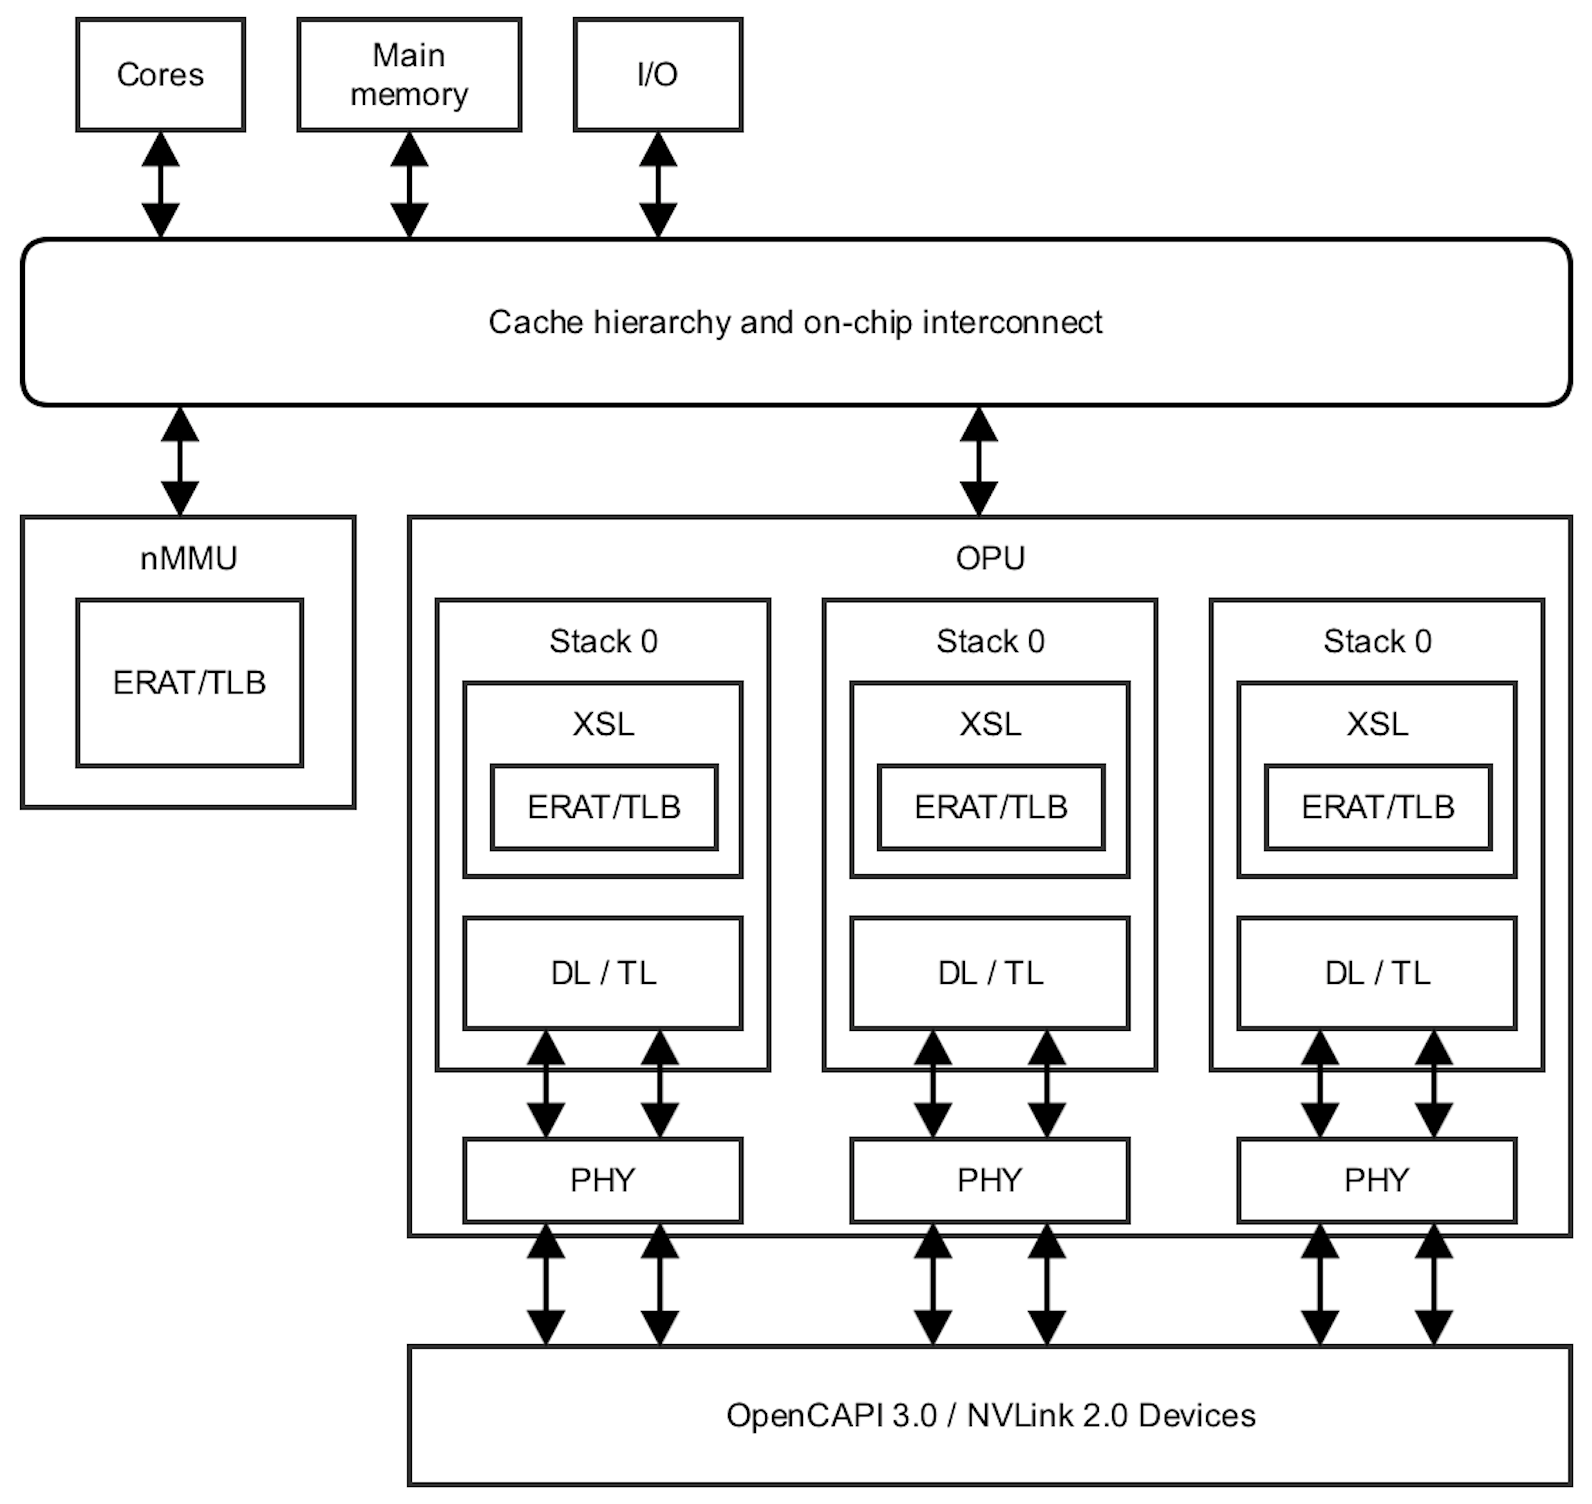
\includegraphics[width=1.0\linewidth]{2-ocapi-host-2.png}
%    \caption{POWER9 architecture specific.}
%    \label{fig:2-ocapi-host-2}
%  \end{subfigure}
%  \caption{System level view of OpenCAPI enablement on the host using the CAPP.}
%  \label{fig:2-ocapi-host}
%\end{figure}

\begin{figure}[htb!]
\ffigbox[\textwidth]
  {
    \begin{floatrow}
    \ffigbox[\linewidth]
      {\captionof{subfigure}{Host architecture agnostic.}
      \label{fig:2-ocapi-host-1}}
      {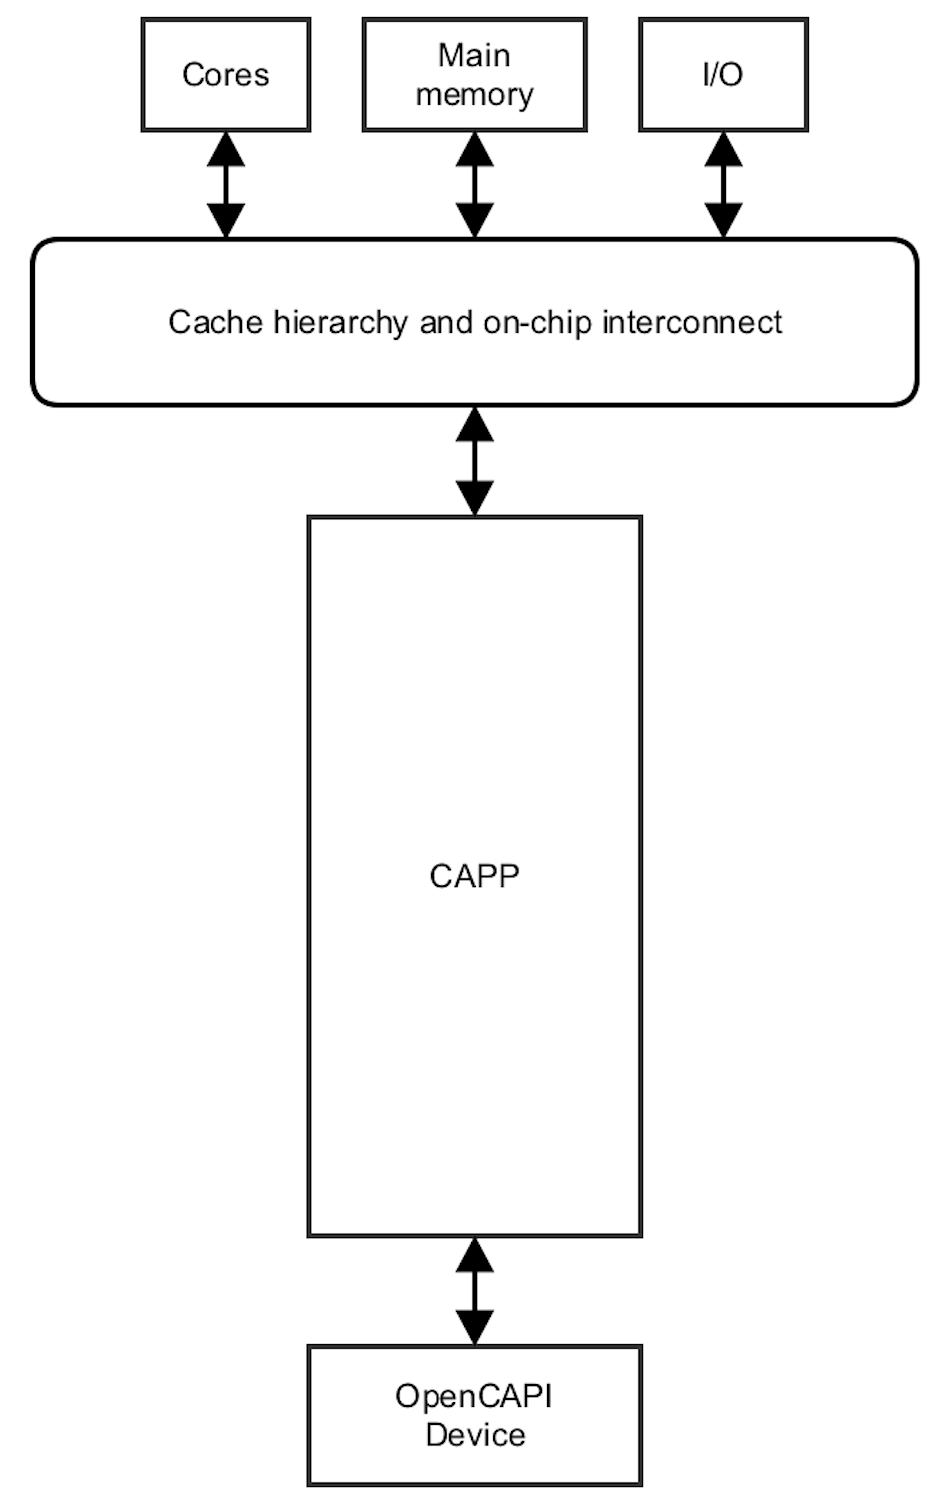
\includegraphics[width=0.50\linewidth]{2-ocapi-host-1.png}}
    \ffigbox[\linewidth]
      {\captionof{subfigure}{POWER9 architecture specific.}
      \label{fig:2-ocapi-host-2}}
      {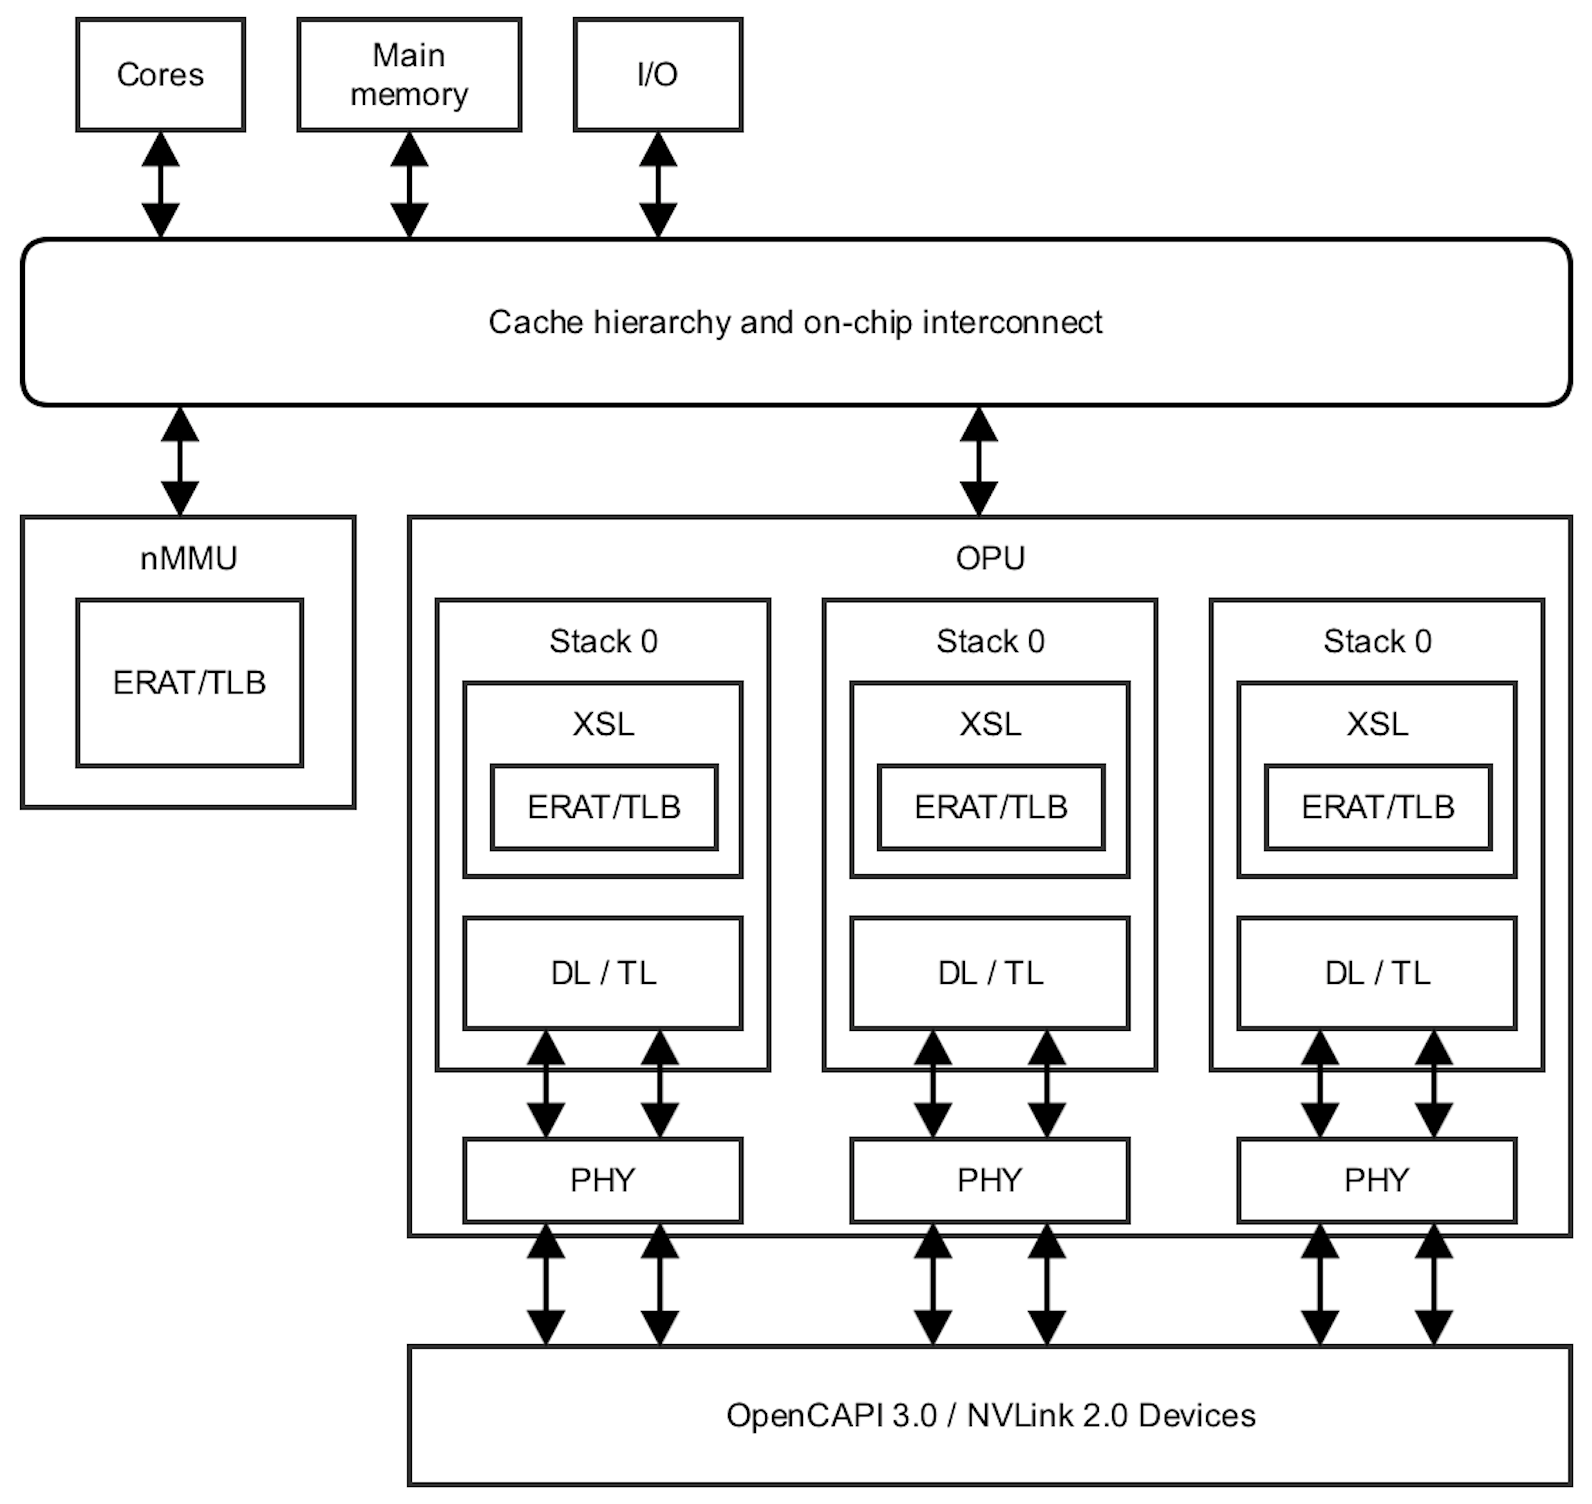
\includegraphics[width=0.85\linewidth]{2-ocapi-host-2.png}}
    \end{floatrow}%
  }
  {\caption{System level view of OpenCAPI enablement on the host using the CAPP.}\label{fig:2-ocapi-host}}
\end{figure}



\subsection{OpenCAPI Attached Device}
\label{sec:cacheline}
The CAPP is provided by the host architecture. On the FPGA side, the physical layer is supplied by the FPGA card vendor. Both the DLX and TLX are implemented using configurable resources on the FPGA and a reference design is provided by the OpenPOWER Foundation. The APL is an optional layer between the TLX and the AFU. Based on experience and customer feedback of CAPI 1.0 \cite{curt}, the OpenCAPI consortium decided to supply no specific interface between the TLX and APL in the sense that there is no cache or buffer present that the AFU can talk to directly. Instead, it provides an interface where TL packet opcodes can be sent to or received from the host.\\
\autoref{fig:2-ocapi-tlx} shows the presented TLX interface from a high level \cite{curt}. The TLX consists of a framer and parser, just like the TL. The parser receives frames from the DLX, unpacks the TL packets and splits the command and response packets, each presented at a separate interface. Each of these two interfaces consists of parsed control information from each TL packet and corresponding data payload. The data payload interface is 64 bytes wide, the same size as a data flit. If the payload of a single TL packet is more than one data flit, it takes multiple cycles to receive the entire data payload. The framer has similar interfaces, but packs TL packets instead to form control flits. There is also a configuration module present on the AFU which holds registers for configuration of the TLX. For example, to enable certain packing templates. There are separate interfaces for this module, not shown in the figure. The TLX also manages credits and each interface has a credit interface in opposite direction. The TLX parser also gives credits back to the TLX framer.\\
The latest generation of Xilinx FPGAs are used that allow an increased operating frequency of up to \SI{450}{\mega\hertz}. To minimize latency, the target frequency of the DLX and TLX is \SI{400}{\mega\hertz}. Each of the four data interfaces can supply up to 64 bytes per cycle at the target frequency. Typically, highly pipelined FPGA designs can reach up to \SI{250}{\mega\hertz}. If an AFU operates at \SI{200}{\mega\hertz}, it will seem like OpenCAPI provides 128 bytes per cycle. This is also the size of a cache line in the POWER architecture.

\begin{figure}[H]
  \centering
  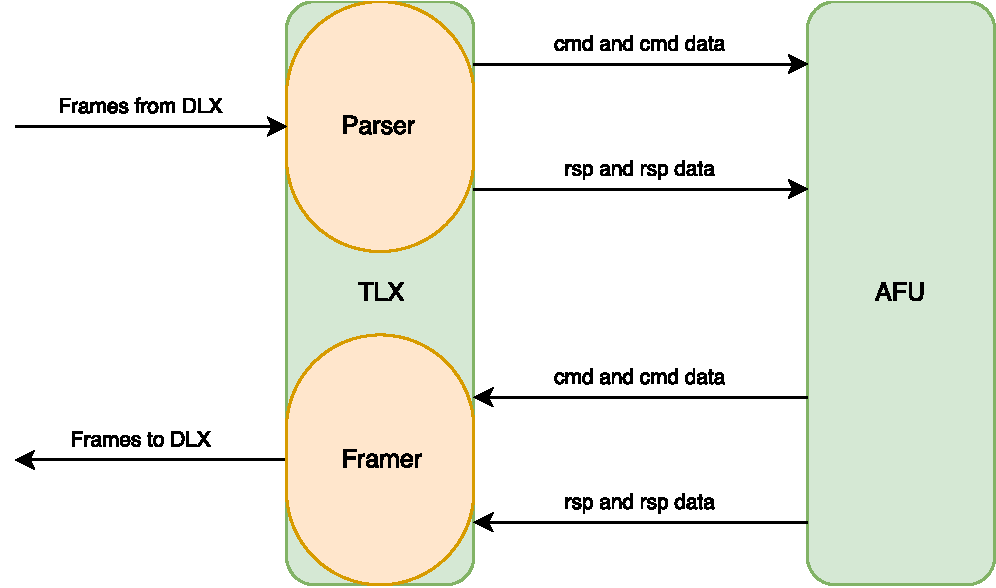
\includegraphics[width=0.55\textwidth]{2-ocapi-tlx.pdf}
  \caption{Interface between the TLX and APL or AFU, depending on the AFU design.}
  \label{fig:2-ocapi-tlx}
\end{figure}

An OpenCAPI device may have three physical address spaces. The configuration space is in a separate space from the MMIO and system memory spaces. These spaces share a PA space and the host can differentiate between the two since the system memory space always starts at offset zero of the PA, while the MMIO space starts at a fixed configured offset from zero. The MMIO offset is configured using a BAR (Base Address Register) and multiple BARs are present to service multiple attached devices.
\begin{itemize}
  \item{\textbf{Configuration space} may be used for configuring the TLX or AFU. It is accessed by using the dedicated read and write commands. A reference configuration space module will be provided by the OpenCAPI consortium.}
  \item{\textbf{MMIO space} may be used for configuration of the AFU and is mapped in the system memory address space.}
  \item{\textbf{System memory space} is a memory space owned by the OpenCAPI device and is mapped to the system's RA space. This memory is coherently accessed using the load/store model used by the host.}
\end{itemize}

A typical usage model is to write a work pointer in an AFU MMIO register or by communication through shared memory. The MMIO module is flexible in the sense that the MMIO base address register and sizes can be configured by the AFU designer. Also configuration registers are present on a per-process basis. The MMIO module is provided by the OpenCAPI consortium and can be integrated directly within a design.

%The following is from section 1.5 in the TL 3.1 tion.

%The configuration space is accessed by using the dedicated read and write commands. The PA specified for this space is separate from the system memory space and the MMIO space. The host may:
%- Provide a configuration address BAR to access this space using a direct access load/store model.
%- Provide an MMIO register set to access this space using an indirect access method.

%The MMIO space shares the PA space used by the system memory space. It is specified by a fixed offset from PA 0 specified in the OpenCAPI device’s configuration space. The host differentiates the MMIO spaces of different OpenCAPI devices by providing a configuration address BAR for each attached device.

%The system memory space is memory space owned by the OpenCAPI device that is mapped to the host’s system memory. The PA for system memory space is defined to start at offset 0. The host differentiates between the different system memory spaces of different OpenCAPI devices by providing a configuration address BAR for each attached device.

%Real addresses (RA) are mapped into the physical address (PA) space specified for a device. This eliminates any requirement placed on the OpenCAPI device to have knowledge of the host’s real address space or how the OpenCAPI device’s PA space is mapped into it. The following rules place restrictions on the OpenCAPI device’s specification of its PA space.



\subsection{Address Spaces and Translation}

%\todo{- Why are there three levels of address translation? RA, EA and PA. Spec talks about function 'convert2PA'. Does the CAPP/OPU have RA2PA translation?\\
%- Curt: are there opcodes for warming up the TLB? I think Andy once mentioned that it is stupid that the TLB(s) are not warmed up during system start-up. TL spec: warming up = The process of loading or populating a cache with a set of valid data.\\
%- Curt: POWER uses three types of addresses. EA, RA and PA. Where does the translation from one to another happen (specifically, where in the drawing)?
%The AFU only uses an EA.  The nMMU translates an EA to an RA internally.  The PA is the physical address in memory (mapped to specific location in a DIMM by the memory controller).\\
%- A program on the P9 or the AFU only see an Effective Address EA for addressing the system address map for OCAPI 3.0 when it masters commands.  If the program wanted the AFU to fetch memory from a DIMM is would give it an EA.  The AFU sends the EA across the link.  The XSL translates the EA to a Real Address (RA).  To do this first it looks in its ERAT.  If it misses the XSL ERAT it forwards the request to the nMMU.  The nMMU will look in its ERAT before walking the page table to resolve the translation into a RA.  The RA is what the fabric bus uses to communicate with caches and DIMM memory.  Physical Address (PA) would be what the memory controller resolves to a physical DIMM address.  An MMU translates an EA to RA via page/segment table walking.  The nMMU handles it for nest units, and the cores have their own MMU as well.  The ERAT is just a TLB that is searched before invoking a page table walk.\\
%- I meant it only uses an EA for mastering commands to memory.  The PA you mention is for slave commands.  That is a PA within the AFU address space (either config or MMIO).  It represents a physical address within the AFU (most likely register).  Some other program accessed this with an EA that was translated to an RA.  The RA matched a range within the NPU that configured it as AFU memory.\\
%- The entire system address map is based on Real Addresses.  That entire map consists of physical DIMM memory (main system memory), PCIe memory, GPU memory, etc.  Each of the regions has a base/size region of the RA that maps to it.  You can think of the physical address as the RA minus the base so it maps directly to a location within the memory device.\\
%}

While address translation is present on the host and managed by hardware, it is of interest to the AFU designer since it can greatly influence performance regarding translation misses. Page table walks are very expensive and take many cycles to complete \cite{curt}. Therefore tuning the AFU to optimally use the TLB and warming up the TLB is a good practice.



\subsubsection{Address Spaces in the POWER Architecture}
\label{sec:spaces}

%\todo{- Curt: Have some figure to show how EA, RA and PA are converted/translated into each other.}

Three different address spaces exist in the OpenCAPI and POWER architecture.
\begin{itemize}
  \item{\textbf{Effective Address (EA)} is the address seen by a program, also known as a virtual address.}
  \item{\textbf{Real Address (RA)} is the address used to access the entire system address map. The entire map consists of physical DIMM memory, PCIe memory, GPU memory, etc. Each of the regions has a base and size region of the RA that maps to it. These addresses are for example used within the fabric on the POWER9 to communicate between caches and DIMM memory.}
  \item{\textbf{Physical Address (PA)} is the address used by a physical memory source, such as a DIMM or local memory of an attached device. You can think of the physical address as the RA minus the base. It maps directly to a location within the memory device.}
\end{itemize}

%From TL spec 3.1:
%EA = Effective address. This is the address as seen by a program. Some host architectures refer to this as a virtual address (VA). Mapping from an EA to an RA requires address translation services.
%RA = Real address. A real address is the result of address translation of an EA. Some host architectures refer to this as a physical address.
%PA = Physical address. This refers to the address space owned by an AFUM device. The host converts the RA to the AFUM device’s physical address space using configuration settings in the host that are deter- mined during initialization of the attached OpenCAPI device.
%A PA is not the result of address translation of an EA as might be the case in some host architectures. The host maps the device’s PA into its own (RA) address space.

The system memory address space includes all addresses within the system and uses real addresses. Main memory is the portion that is normally backed by physical DIMMs and marked coherent. This can be cached by processor caches and coherency maintained. MMIO (memory mapped I/O) is mapped into the system memory map, but it is marked in the page tables as non-cacheable. This includes the PCI Express devices MMIO regions, AFU MMIO regions, as well as the processor MMIO addresses. MMIO regions consist usually of registers and are used for configuration of the system and communication with the device driver for I/O devices. It is a region in the system memory map because it is accessed across the fabric from a program running inside a core to communicate with the attached device via EA-RA translation.



\subsubsection{Address Translation}
Taking a look at \autoref{fig:2-p9-system} again, the fabric uses real addresses. If a memory location within a DIMM is accessed, the memory controller resolves a physical address from the real address. Cores have their own MMU in order to translate an effective address to a real address via page/segment table walking. An effective address will be translated to a real address if a memory location has to be accessed outside of the current core.\\
In OpenCAPI, all translations happen on the host and occur either in the OPU or nMMU. In CAPI 1.0, part of the translation was located on the FPGA (in the PSL). Moving the address translation to the host reduces design complexity of attached devices. Since an attached device never has access to a physical address, malicious attached devices are not able to access unauthorized memory locations, such as addresses belonging to kernel or other applications.\\
The AFU only uses effective addresses for mastering commands to host memory, that are translated on the host to real addresses. When the AFU acts as a slave and receives commands from the host, physical addresses are used to access the three different physical address spaces mentioned in Section \ref{sec:spaces}. These physical addresses have been translated from program EA, to system RA, to PA. The host converts the RA to a PA using configuration settings in the host that are determined during initialization of the attached OpenCAPI device.\\
Real addresses are mapped into the physical address space specified for an OpenCAPI device. This eliminates any requirement placed on the OpenCAPI device to have knowledge of the host’s real address space or how the OpenCAPI device’s PA space is mapped into it. The PA for CAPP commands is all translated in the host (MMIO, Config, host memory). The host has programmable base address (BAR) and offset registers for everything. The PA space in the FPGA is either config space (indicated by command type), MMIO (indicated by matching the AFU's base address), or host memory (if it doesn't match the AFU's BAR).

% Mastering commands means AFU is 'master' of the interconnect. So when it sends out TL command packets.
% When the AFU acts as a slave, it services host commands.



\subsubsection{Address Translation Example}
As an example, consider a POWER9 with an OpenCAPI-attached device. A program on the processor only sees an Effective Address for addressing the system address map. If the program requests the AFU to fetch data from host memory it uses an EA. The AFU sends the EA across the OpenCAPI link and the XSL translates the EA to a Real Address (RA). To do this, first it looks in its ERAT. If it misses the XSL ERAT it forwards the request to the nMMU. The nMMU will look in its ERAT before walking the page table in host memory to resolve the translation into an RA. If the page walk fails it will return a bad status to the OPU, and it will generate a fault interrupt to resolve the fault.\\
In the other direction, a program uses an EA and the OS sets up mappings between a page to a physical resource. To communicate across the fabric, the program EA is translated to an RA. The RA is then matched to a range within the OPU that is configured as AFU memory and translated from RA to PA.



\section{Coherent Programming Model}
%\todo{
%- No cache coherence: a solution would be to implement coherency is software, but that introduces a lot of overhead. to cover the latency a solution has to be found. a local mem on the fpga is needed. how to move data to it? following stuff in requirements: accelerators like database operators can operate under the offload paradigm.\\
%}

OpenCAPI enables new, easier and more natural programming models, as found on multi-core systems, for IO that was not possible with the traditional approach. Attached devices are more easily accessible due to the shared virtual memory space and appear as peers to the processor cores. Also the setup and completion phases, by interacting with device drivers, have been simplified and made faster. Combining this with attaching devices with a low-latency interconnect, the attached devices become tightly coupled that allows for thread-level parallelism between the application running on the host and the attached device.



\subsection{Coherent Shared Virtual Memory}
The approach of OpenCAPI (and CAPI for that matter) offers a virtual address space shared between the processor caches and the attached device \cite{opencapi-jeff-preso}. The host and accelerator can coherently access each others physical memories. This removes the problem of having multiple copies of the same data in a traditional IO model (see Section \ref{sec:copies}) and reduces setup and completion time significantly for an application wanting to use the attached device. Typically, this might take \SI{12.8}{\micro\second} as shown in \autoref{fig:2-flow-model}. Now it might take as little as \SI{0.36}{\micro\second}.\\
Not only can the host use atomic operations, but also the attached device has a vast set of atomic operations to implement synchronization operations. A special wake host thread opcode can be used for communication as well.\\
%OpenCAPI is also flexible in configuration. If the attached device does not want to support atomics for example, you tell the host and atomics will be send out as special read and write operations.\\
The shared virtual memory space also allows programmers to dereference pointers everywhere, while previously host pointers could only be dereferenced on the host and vice versa \cite{benton}. This removes the manual movement of data between the host and attache device. Overall it simplifies the programming model since the attached device operates as a peer to the other processor cores. With the traditional IO model, sharing an attached device between applications was difficult because pinned memory belongs to only one application and cannot be shared. If the attached device supports multiple hardware buffers, multiple applications could use the device. The number of applications is dependent on the hardware. OpenCAPI allows for sharing the accelerator between applications due to a special feature in the standard (context bits).\\
With CAPI, a coherent cache was present on the accelerated device. This allows for even more programmer flexibility and lower latency for highly referenced data. However, this feature is absent in OpenCAPI 3.0 but will return in OpenCAPI 4.0.

%\todo{- Make own figures (two subfigures).}

\begin{figure}[H]
  \centering
  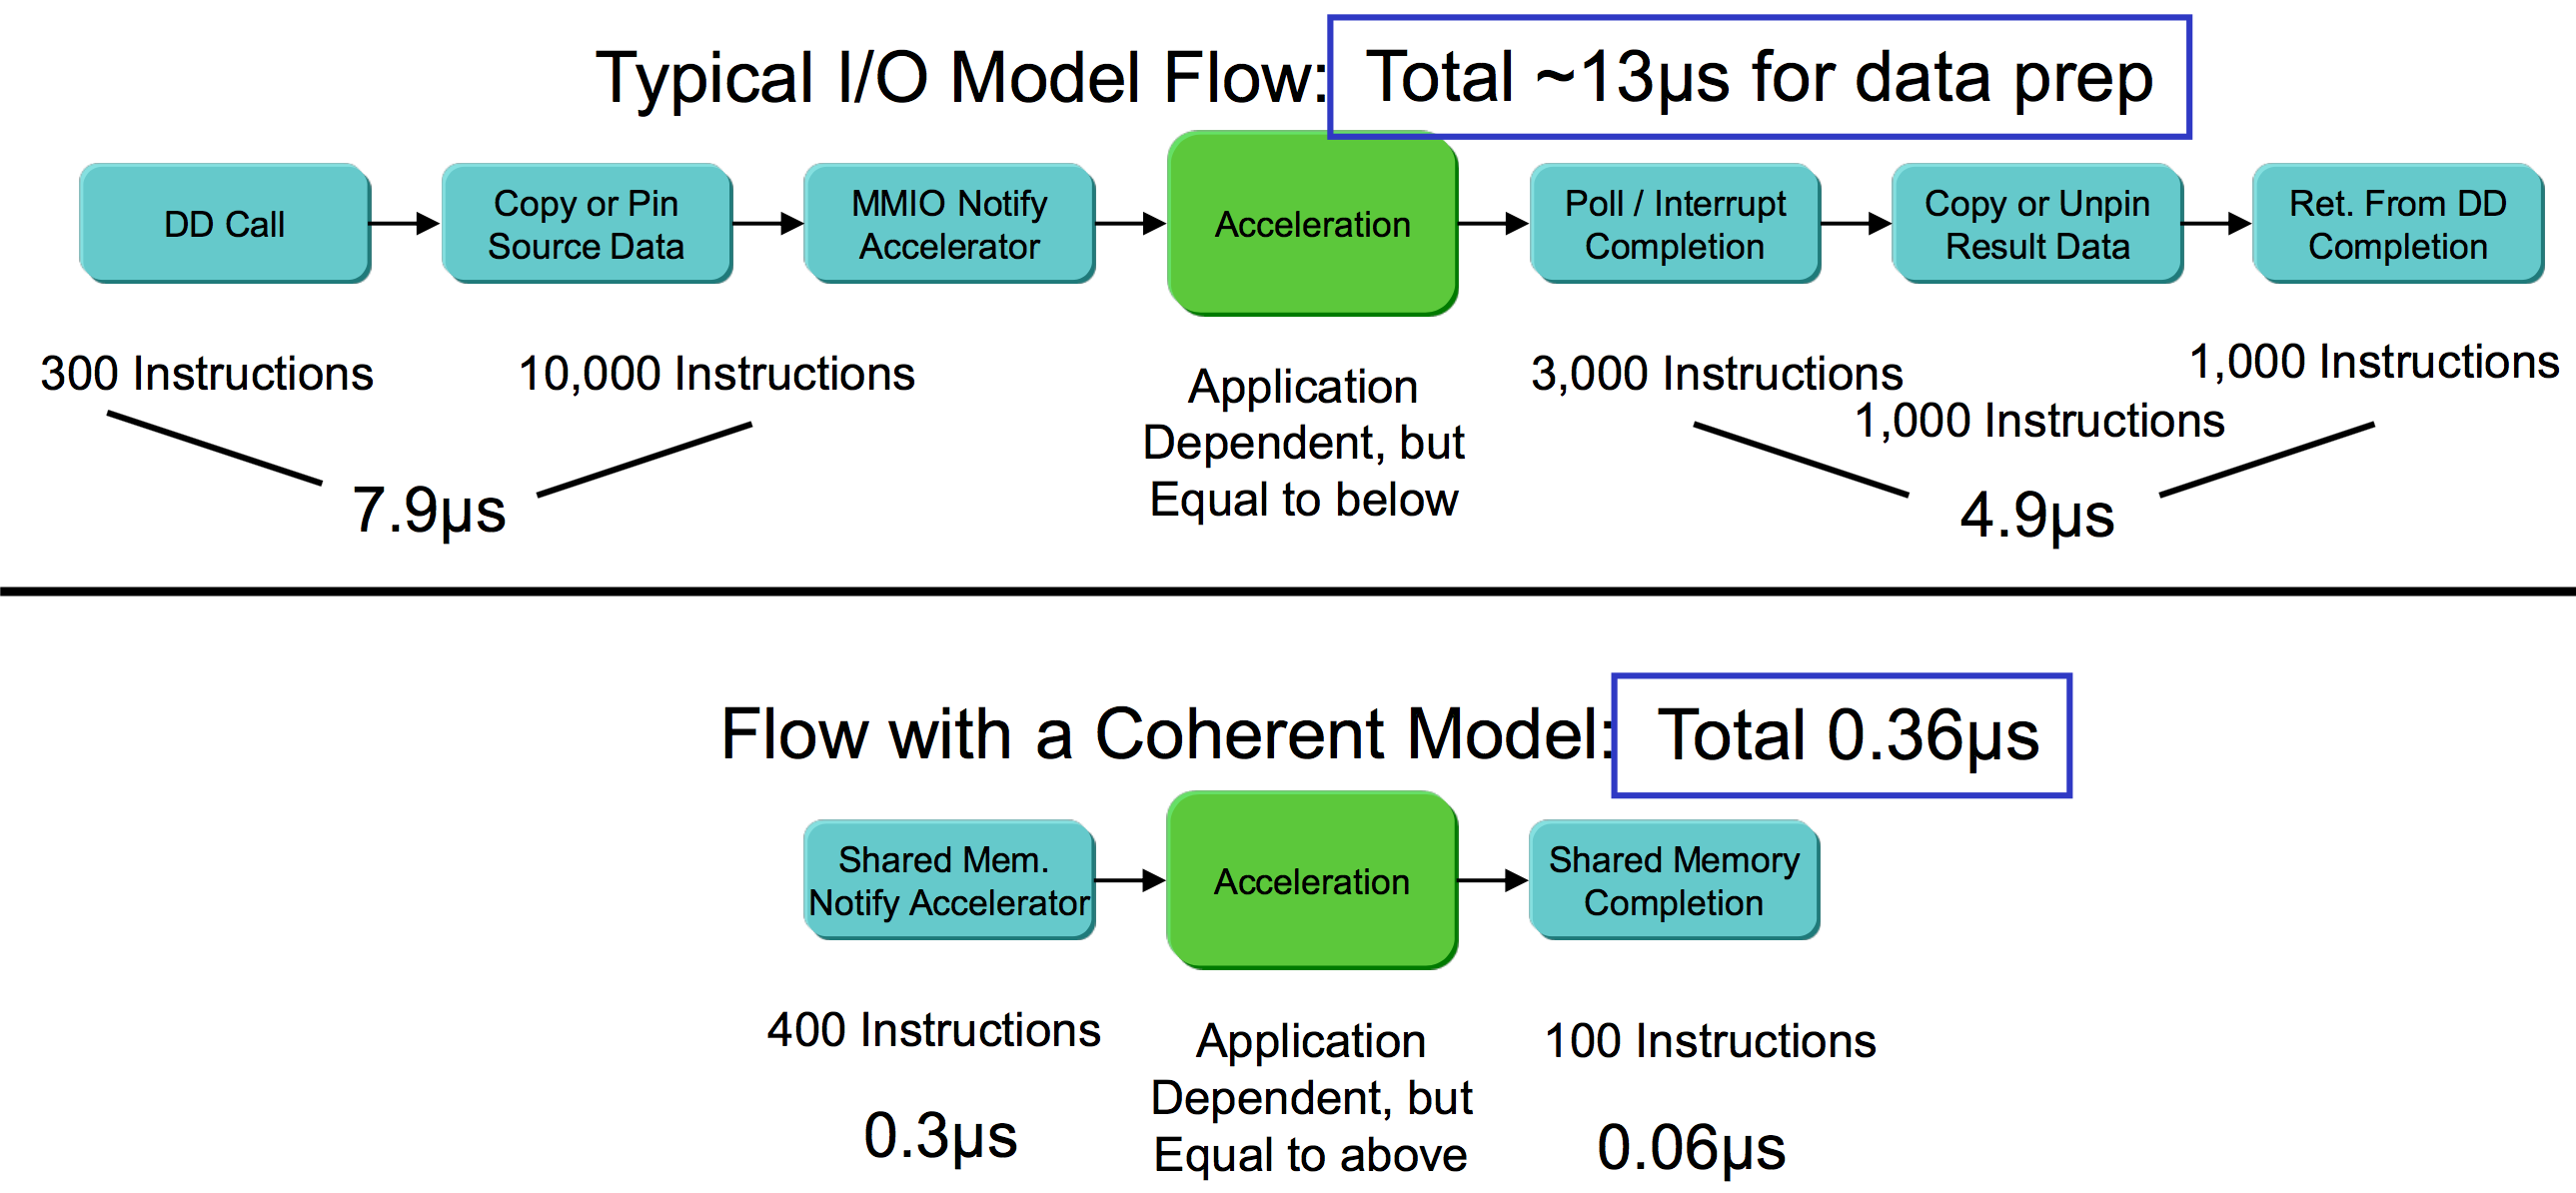
\includegraphics[width=0.80\textwidth]{2-flow-model.png}
  \caption{Traditional IO device setup and completion flow versus the OpenCAPI flow \cite{opencapi-enablement}.}
  \label{fig:2-flow-model}
\end{figure}



\subsection{Accelerator Paradigms}
Traditionally, an offload paradigm was used for accelerators, shown in \autoref{fig:2-ocapi-paradigm-1}. \autoref{fig:2-ocapi-paradigm} shows current and new paradigms enabled by OpenCAPI. A perfect example is an application that uses pointer chasing or linked lists \cite{opencapi-forum}. This was not possible because pointers were not able to be dereferenced since the processor and IO device did not share the same address space. Other applications could include using both the shared host memory and local memory of the accelerator, since accessing host memory has a very low latency. An example of such a bi-directional accelerator is shown in \autoref{fig:2-ocapi-paradigm-5}.

\begin{itemize}
  \item{\textbf{Memory transform} is the traditional offload paradigm. GPUs fall into this category.}
  \item{\textbf{Needle-in-a-haystack engine} processes a large data set from disk for example and filters specific data of interest.}
  \item{\textbf{Egress transform} processes outgoing data, as it leaves the system. Examples are compression and encryption on its way to centralized storage.}
  \item{\textbf{Ingress transform} processes incoming data, for example from a NIC, and places the output in host memory. An example could be decompression and decryption.}
  \item{\textbf{Bi-directional transform} can be used for a hash-join database operator using a database located on disk. The hash table can be build in host processor memory. Stream through data from disk and do computations that while fetching hash table from host memory.}
\end{itemize}

\begin{figure}[H]
  \begin{subfigure}{.5\textwidth}
    \centering
    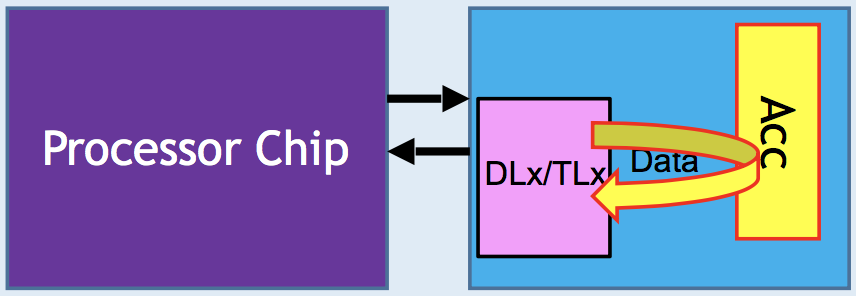
\includegraphics[width=0.90\linewidth]{2-ocapi-paradigm-1}
    \caption{Memory transform.}
    \label{fig:2-ocapi-paradigm-1}
  \end{subfigure}%
  \begin{subfigure}{.5\textwidth}
    \centering
    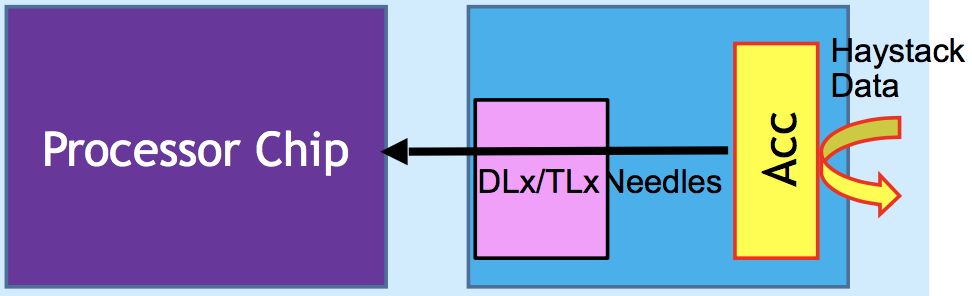
\includegraphics[width=0.95\linewidth]{2-ocapi-paradigm-4}
    \caption{Needle-in-a-haystack engine.}
    \label{fig:2-ocapi-paradigm-4}
  \end{subfigure}\\[1ex]
  \begin{subfigure}{.5\textwidth}
    \centering
    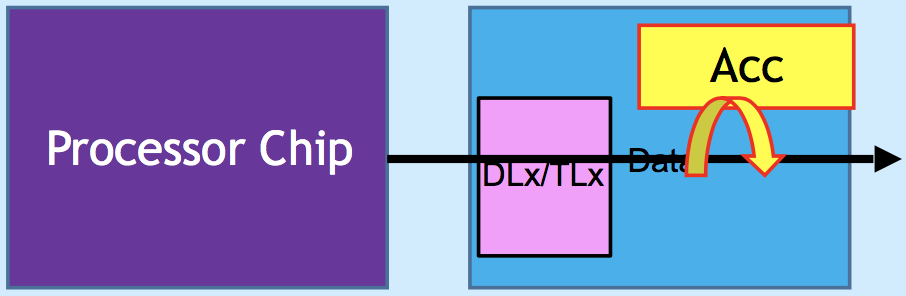
\includegraphics[width=0.90\linewidth]{2-ocapi-paradigm-2}
    \caption{Egress transform.}
    \label{fig:2-ocapi-paradigm-2}
  \end{subfigure}%
  \begin{subfigure}{.5\textwidth}
    \centering
    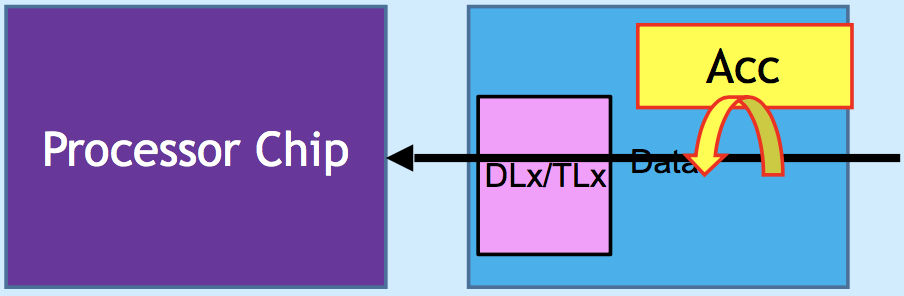
\includegraphics[width=0.95\linewidth]{2-ocapi-paradigm-3}
    \caption{Ingress transform.}
    \label{fig:2-ocapi-paradigm-3}
  \end{subfigure}\\[1ex]
  \begin{subfigure}{\textwidth}
    \centering
    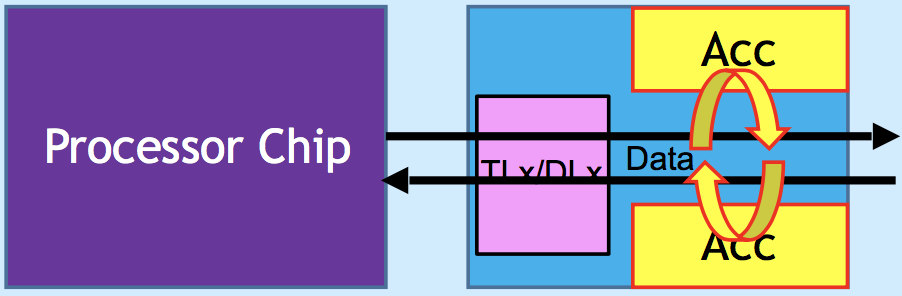
\includegraphics[width=0.45\linewidth]{2-ocapi-paradigm-5}
    \caption{Bi-directional transform.}
    \label{fig:2-ocapi-paradigm-5}
  \end{subfigure}
  \caption{Accelerator paradigms enabled by OpenCAPI \cite{opencapi-jeff-preso}.}
  \label{fig:2-ocapi-paradigm}
\end{figure}





\section{FPGA Characterization}
\label{sec:fpga-characterization}
FPGAs are integrated circuits that can be reconfigured after fabrication (field programmable). A lot can be said about FPGAs and their operation, but the focus of this section is to provide background information for those aspects of FPGAs that most directly relate to the implementation of the proposed architecture. The background information provided in this section will be used throughout the rest of the thesis.



\subsection{FPGA Architecture}
\label{sec:fpga-arch}
Typically, FPGAs consist of arrays of programmable logic blocks that can be wired together. Logic blocks can be used to implement combinatorial logic, by configuring look-up tables (LUTs), or to implement sequential logic such as flip-flops and small memories. Besides configurable blocks, also hardwired logic is present such as multiplexers, special DSP slices, networking stacks, and PCI Express controllers.\\
\autoref{fig:2-fpga-arch} shows the physical architecture of an FPGA. The most common resources such as IO Blocks, CLBs, memories, and DSP Blocks are shown. What is important to notice is that each type of resource is located in a separate column. Memories for example could be located relatively far away from where their data is processed. Depending on the target frequency of the design, wire delays could start to play a large role. When routing within a single clock cycle fails, additional registers are required between a memory and the data consumer. For this reason, memory primitives typically contain one or multiple additional pipeline stages within the primitive to help with routing, at the cost of increased latency.

\begin{figure}[H]
  \centering
  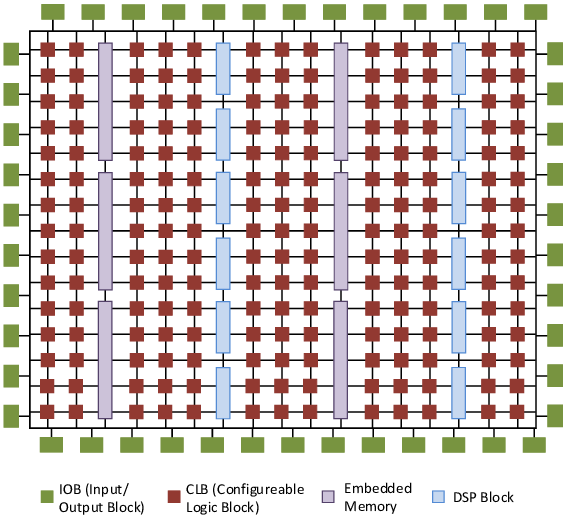
\includegraphics[width=0.50\textwidth]{2-fpga-arch.png}
  \caption{Diagram showing the physical architecture of an FPGA \cite{fpga-fig}.}
  \label{fig:2-fpga-arch}
\end{figure}



\subsection{Typical Resources}
We study two Xilinx FPGAs for their suitability to be used as OpenCAPI accelerators. Both FPGAs, the KU15P and VU37P, are from the latest UltraScale+ architecture and are the highest model in each device family, Kintex+ and Virtex+, respectively. Compared to previous architectures, UltraScale+ adds Ultra RAM (URAM). This memory resource falls in between the typical BRAM and DRAM capacities, and High Bandwidth Memory (HBM) Gen 2 for the top tier Virtex+ FPGAs. Table \ref{tab:fpga} shows a summary of specifications for both FPGAs. The GTY transceivers mentioned in the table have a maximum bandwidth of \SI{32.75}{\giga\bit\per\second}, which is more than that of the OpenCAPI lanes at \SI{25}{\giga\bit\per\second}. The table shows that both FPGAs can easily handle eight lanes to attach to OpenCAPI. The following itemization explains most of the specifications in more detail. It is important to note that the VU37P excels in every aspect compared to the KU15P.
\begin{itemize}
  \item{\textbf{CLB flip-flops} reports the number of flip-flops across all CLBs in thousands.}
  \item{\textbf{CLB LUTs} reports the number of LUTs across all CLBs in thousands.}
  \item{\textbf{Distributed RAM} reports the maximum memory capacity.}
  \item{\textbf{BRAM} reports the total memory capacity, both with and without ECC support.}
  \item{\textbf{URAM} reports the total memory capacity, both with and without ECC support.}
  \item{\textbf{HBM} reports the total available HBM capacity on the FPGA.}
  \item{\textbf{DSP slices} reports the number of available DSP slices on the FPGA.}
  \item{\textbf{GTY transceivers} reports the total number of \SI{25}{\giga\bit\per\second} transceivers available.}
\end{itemize}

\begin{table}[h]
  \centering
  \caption{Specification summary of the Xilinx KU15P and VU37P FPGAs \cite{xilinx-fpga}.}
  \label{tab:fpga}
  \begin{tabular}{ l | c | c }
    \textbf{Resource}               & \textbf{KU15P}  & \textbf{VU37P} \\ \hline
    %System logic cells (K)          & 1143            & 2852 \\
    CLB flip-flops [k]              & 1045            & 2607 \\
    CLB LUTs [k]                    & 522             & 1304 \\
    %Number of distributed RAMs      & 161280          & xxx \\
    Distributed RAM capacity [Mb]   & 9.8             & 36.7 \\ % KU15P = 161280 * 64b / 8b/B
    %Distributed RAM [Mb]            & 9.8             & 36.7 \\
    %Number of BRAMs                 & 984             & 1968 \\
    BRAM capacity with ECC [Mb]     & 34.6             & 70.9 \\ % KU15P = 512*72*984/8
    BRAM capacity without ECC [Mb]  & 30.8             & 63.0 \\ % KU15P = 512*64*984/8
    %Total block RAM [Mb]            & 34.6            & 70.9 \\
    %Number of URAMs                 & 128             & \\
    URAM capacity with ECC [Mb]     & 36.0             & 270.0 \\ % KU15P = 4*1024*72*128/8
    URAM capacity without ECC [Mb]  & 32.0             & 240.0 \\ % KU15P = 4*1024*64*128/8
    %Total ultra RAM [Mb]            & 36.0            & 270.0 \\
    HBM capacity [GB]               & 0               & 8 \\
    DSP slices                      & 1968            & 9024 \\
    GTY transceivers                & 32              & 96 \\
  \end{tabular}
\end{table}



\subsection{Configurable Logic Blocks}
\label{sec:clb}
The UltraScale+ architecture consists of an array of Configurable Logic Blocks (CLB), with two distinct flavors \cite{xilinx-ug574}. Each CLB consists of eight six-input LUTs, sixteen flip-flops, and seven hardwired multiplexers to select between LUT outputs if needed. A LUT is used to implement a logic function and each of them is accompanied by two flip-flops and can be configured as either a six-input one-output or a five-input two-output LUT. Besides the hardwired multiplexers, the LUTs can also be used to implement a 4:1 multiplexer by using four inputs for data and two inputs for the selection signal. \autoref{fig:2-xilinx-mux} shows how a 16:1 multiplexer can be implemented in half of a CLB. Similarly, a 32:1 multiplexer can be implemented in a single CLB by using all LUTs and hardwired multiplexers. Internally, a CLB can either be a \textit{SLICEL} or a \textit{SLICEM}. The previously mentioned logic is present in a \textit{SLICEL}. In addition to this, a \textit{SLICEM} can also be configured with up to \SI{512}{\bit} of distributed RAM or with a \SI{256}{\bit} shift register. Distributed RAM can be configured as single, dual, quad, octal or simple dual-port with a minimum memory capacity of \SI{32}{\bit} per primitive up to a maximum of \SI{512}{\bit} per slice with either \SI{1}{} or \SI{2}{\bit} wide data.

\begin{figure}[h]
  \centering
  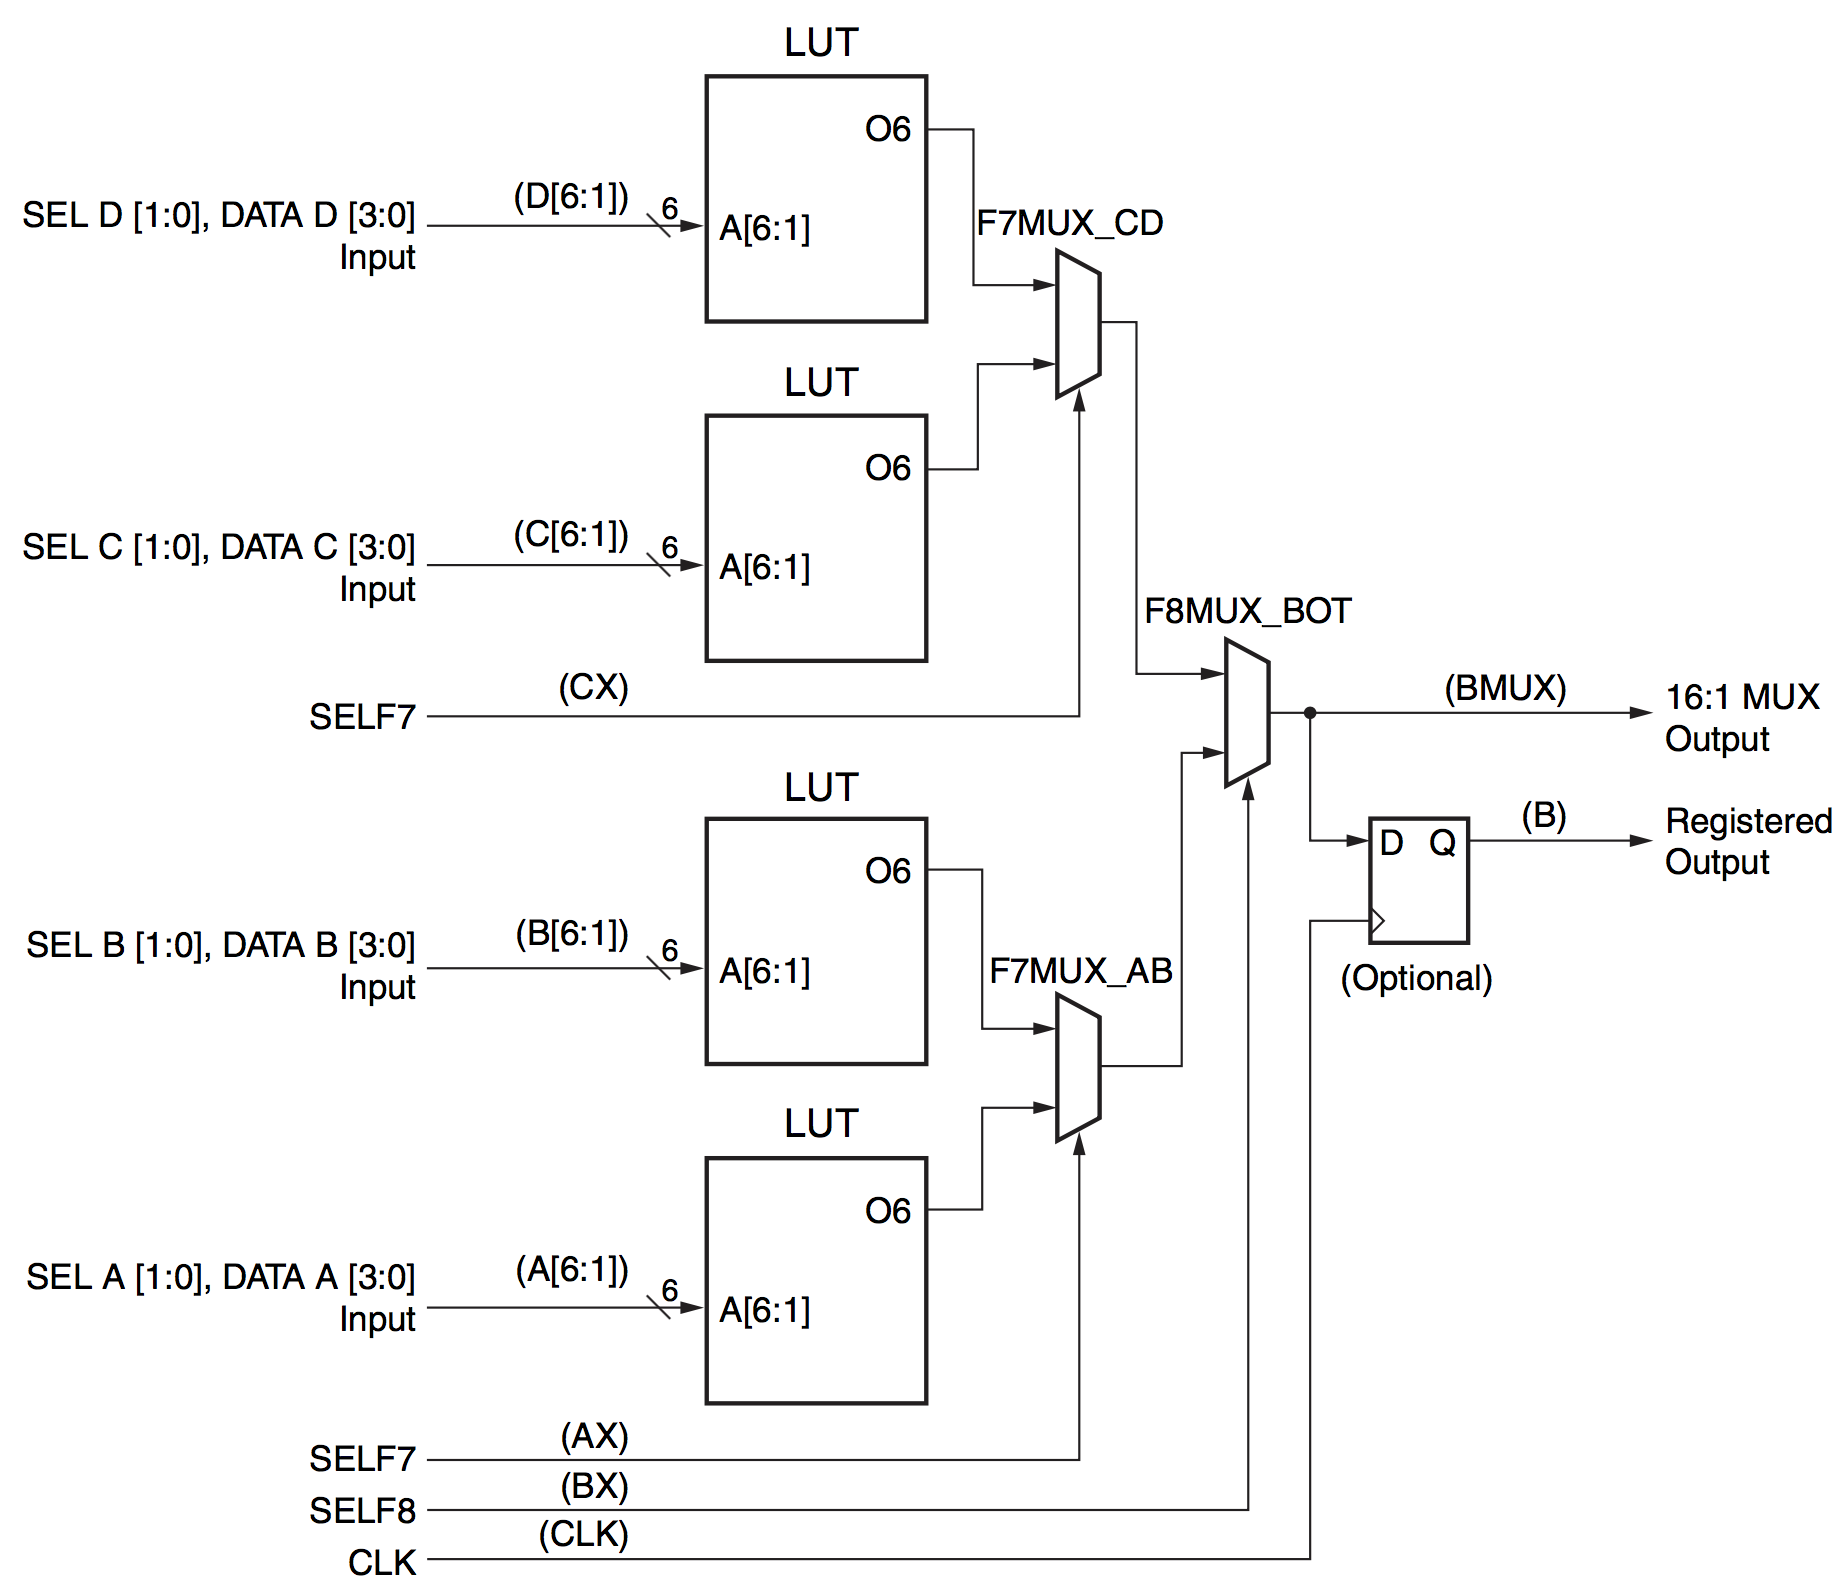
\includegraphics[width=0.70\textwidth]{2-xilinx-mux.png}
  \caption{16:1 multiplexer using half a CLB in the UltraScale+ architecture \cite{xilinx-ug574}.}
  \label{fig:2-xilinx-mux}
\end{figure}



\subsection{Memory Resources}
Several different memory resources exist, either inside or outside of the FPGA. The UltraScale+ architecture brings two additional memory resources to the table: URAM and HBM. The following list is sorted based on increasing memory capacity and latency \cite{xilinx-ug573}.
\begin{itemize}
  \item{\textbf{Distributed RAM} is RAM built from LUTs within a slice and supports several configurations. Multiple read ports are supported, but multiple write ports are not.}
  \item{\textbf{Block RAM} are dedicated RAM primitives with ECC support of \SI{36}{\kilo\bit} in size. The primitive consists of two independent \SI{18}{\kilo\bit} RAMs that can be configured as a Simple Dual Port (SDP) or True Dual Port (TDP) memory. Each BRAM has two independent read and write ports. A \SI{36}{\kilo\bit} BRAM can be configured with independent ports as 32K x 1, 16K x 2, 8K x 4, 4K x 9, 2K x 18 or 1K x 36 for a TDP configuration or additionally as 512 x 72 for an SDP configuration. An \SI{18}{\kilo\bit} BRAM can be configured with the same data widths, but with half of the entries. By default the read latency is one cycle, but an optional read register can be configured.}
  \item{\textbf{Ultra RAM} are also dedicated RAM primitives with ECC support but have a larger capacity compared to BRAM primitives. Two ports are available and one configuration of 4K x 72. A port either operates as a read or write port and port A always completes before port B does. Similarly to a BRAM primitive, optional registers can be configured between one and four cycles of latency.}
  \item{\textbf{HBM} is high-bandwidth memory reaching bandwidths up to \SI{460}{\giga\byte\per\second}. This memory is only supported on top tier Virtex+ FPGAs up to \SI{8}{\giga\byte} \cite{xilinx-hbm}.}
  \item{\textbf{DRAM} is located outside of the FPGA and has a capacity of up to several gigabytes.}
\end{itemize}

%\todo{- add max frequencies of RAMs.\\}



\subsubsection{BRAM Address Collision}
An address collision occurs when both ports of a BRAM primitive access the same address in a single clock cycle. The resulting behavior depends on the port configuration. If both ports read, both accesses complete successfully. If both ports write, the memory location contains non-deterministic data. If one port reads and the other writes, the write data operation completes successfully. The read access is only successful for common clock designs and the write port is configured as read-first \cite{xilinx-ug573}.



\subsubsection{URAM Address Collision}
Similarly, an address collision can also occur for a URAM primitive. When both ports write in the same clock cycle, the port B write takes effect since port A always completes before port B. If port A reads and port B writes, port A receives the old data and the new data is stored at the memory location. If port A writes and port B reads, the new data is written to the memory location and port B reads the new data immediately \cite{xilinx-wp477}.


%- add info about SDP and TDP BRAMs and when collisions occur. see \url{https://www.xilinx.com/support/documentation/ip_documentation/blk_mem_gen/v8_3/pg058-blk-mem-gen.pdf} page 51.\\
%- is BRAM write at most one cycle? should check or test this. according to UG573 page 12 BRAM write operation is always single clock-edge operation. Read uses one or two, depending on if the output register is configured.\\

%Xilinx PCIe Memory Bandwidth - WP464\\
%Using WP464 with 2.5 scaling factor to account for both read and write directions and any additional overhead such as memory addressing. Total memory bandwidth required for sustained transfers:
%\begin{equation}
%  $50GB/s * 2.5 = 125 GB/s = 1000 Gb/s$
%\end{equation}
%Required interface width for DDR4 memory at 2133Mb/s:
%\begin{equation}
%  $1000 Gb/s / 2133Mb/s per pin = \approx 469 pins$
%\end{equation}
%DDR4 memory is supplied in 288-pin dual in-line memory modules (DIMMs).



\subsection{DLX and TLX Reference Design}
\label{sec:dlxtlx}
As mentioned in Section \ref{sec:cacheline}, a DLX and TLX reference design is provided that can be integrated as a module by the AFU designer. Because the reference design is implemented in FPGA logic, care must be taken that both the reference design and the AFU fit inside the specific FPGA resource budgets. \autoref{tab:9v3} shows the resource utilization obtained using Vivado 2017.1 when targeting a Xilinx VU3P FPGA on the Alpha Data 9V3 OpenCAPI-capable card. The number of resources used and the percentage consumed of the total number of resources available are shown. These results are from October 10, 2017 and are subject to change \cite{opencapi-enablement}.

\begin{table}[H]
  \centering
  \caption{Resource utilization for the DLX and TLX layers \cite{opencapi-enablement}.}
  \label{tab:9v3}
  \begin{tabular}{ l | c | c | c }
    \textbf{Resource}   & \textbf{DLX}  & \textbf{TLX}  & \textbf{Total} \\ \hline
    CLB Registers       & 9392 (1.19\%) & 13806 (1.75\%)    & 23198 (2.94\%) \\
    CLB LUTs            & 19026 (4.83\%) & 8463 (2.15\%)    & 27489 (6.98\%) \\
    LUT as Memory       & 0 (0\%) & 2156 (1.09\%)           & 2156 (1.09\%) \\
    BRAMs               & 7.5 (1.0\%) & 0 (0\%)             & 7.5 (1.0\%) \\
  \end{tabular}
\end{table}

%\todo{
%- "Memcopy, Home Agent Memory and AFP exercisers are all up and running cleanly using the Alpha Data 9V3 card with VU3P FPGA"\\
%- 9V3 datasheet in comment % https://www.alpha-data.com/pdfs/adm-pcie-9v3%20user%20manual.pdf
%}
%\todo{
%I remember that ADM might be what you mean (Alpha Data). They have OpenCAPI cards for VU3P. They also said they are going to support one like VU37P.
%}

\section{Preliminary Concluding Remarks}
The bottlenecks present in the traditional IO model are addressed by OpenCAPI and this chapter provided a deeper understanding of this protocol. Additionally, various emerging use cases for attached accelerators are presented. A brief summary of the latest generation of Xilinx FPGAs, compatible with OpenCAPI, is required for the remainder of this thesis. Due to the order of magnitude increase in interconnect bandwidth, new challenge arise for AFU designers. Questions regarding the partitioning of the algorithm, concurrent usage of multiple software threads, and the design of the accelerator come to mind.\\
Another question we can ask ourselves is how the accelerator is fed with data, since no buffer or cache is present on the attached OpenCAPI device by definition. Chapter 5 generalizes across multiple common accelerator memory access patterns and proposes an architecture to keep accelerators fed with data at OpenCAPI-like bandwidths.
